\documentclass[11pt]{article}

\usepackage{fontspec}
\usepackage{microtype}
\usepackage{xltxtra}
\usepackage{polyglossia}
\setdefaultlanguage{marathi}
\setmainfont[Script=Devanagari,Mapping=devanagarinumerals,StylisticSet=1]{Yashovenu}

\setotherlanguage[variant=uk]{english}
\newfontfamily\englishfont{Courier}
\newfontfamily{\Bask}{Baskerville}%OSX
%\newfontfamily{\Bask}{Ubuntu}%Linux

\setotherlanguages{sanskrit,hindi,tamil, bengali, kannada, malayalam}
\newfontfamily\sanskritfont[Script=Devanagari, Mapping=devanagarinumerals]{Sanskrit 2003}
\newfontfamily\hindifont[Script=Devanagari,
Mapping=devanagarinumerals]{Mukta}
\newfontfamily\tamilfont{Arial Unicode MS}%OSX
\newfontfamily\bengalifont{Arial Unicode MS}%OSX
\newfontfamily\kannadafont{Arial Unicode MS}%OSX
\newfontfamily\malayalamfont{Arial Unicode MS}%OSX
% \newfontfamily\tamilfont{Lohit Tamil}%Linux
% \newfontfamily\bengalifont{Lohit Bengali}%Linux
% \newfontfamily\kannadafont{Lohit Kannada}%Linux
% \newfontfamily\malayalamfont{Lohit Malayalam}%Linux


 \newfontfamily{\Yvenu}[Script=Devanagari]{Yashovenu}
 \newfontfamily{\Mukta}[Script=Devanagari]{Mukta}
 \newfontfamily{\Sharad}[Script=Devanagari]{Sharad76}
 \defaultfontfeatures{Ligatures=TeX}

 \usepackage{textcomp}
 \usepackage{verse}
 \usepackage{dramatist}
 \usepackage{hyperref}
 \usepackage{color}
 \usepackage[inline, shortlabels]{enumitem}
 \usepackage{dirtytalk}

 \usepackage{makeidx}
 \makeindex

 \usepackage[top=2cm, left=2cm, right=1.6 cm, bottom=2.2cm]{geometry}

%newcommands
\newcommand{\7}{\textbackslash}
\newcommand{\Syn}{\textenglish}
\newcommand{\attrib}[1]{%
 \nopagebreak{\raggedleft\normalfont #1\par}}%for package verse

 \renewcommand{\scenename}{दृश्य}%for dramatist
 \renewcommand{\thescene}{\arabic{scene}}%for dramatist

\renewcommand\UrlFont{\ttfamilylatin}%for url
\gappto\captionsmarathi{\renewcommand{\figurename}{चित्र}}

\begin{document}

\thispagestyle{empty}

\title{लाटेक् आणि पॉलिग्लॉसियाची ओळख\\ {\small आवृत्ती क्र १.० ({\Bask Version 1.0})}}
\author{रोहित दिलीप होळकर \thanks{\Bask Copyright {\textcopyright} \@
 2017 Rohit Dilip Holkar; LaTeX Project Public Licence; see the last page for details.}}
 \date{}
\maketitle

\begin{abstract}
मराठीकरिता लाटेक् आणि लाटेक्-चे हे पॉलिग्लॉसिया पॅकेज कसे वापरावे हे शिकवणारी ही
हस्तपुस्तिका आहे. थोडेफार फेरबदल करून ही पुस्तिका संस्कृत, हिंदी आणि इतर भारतीय
भाषांकरिताही वापरता येणे शक्य आहे; हे फेरबदल काय असावेत हे
विभाग~\ref{sec:first-doc}मध्ये स्पष्ट केले आहे. प्रस्तुत पुस्तिकेची ही आवृत्ती क्र १.० आहे. 
\end{abstract}
\vspace{0.5in}

\begin{center}
{\Bask \bfseries English summary}
\medskip

 {\Bask English title:{\itshape A practical guide to {\LaTeX} and
     polyglossia for Indian Languages,} Version 1.0
\smallskip

Author: {\itshape Rohit Dilip Holkar}
\smallskip

 Summary:{ This is a short guide to {\LaTeX} and its package
 polyglossia. This document aims to introduce {\LaTeX} and
 polyglossia for Indian languages. Though the document often
 discusses the language Marathi, the discussion applies to other India languages also with some minute changes which are described in Section~\ref{sec:first-doc}. We also discuss some issues in polyglossia for Marathi, Sanskrit and Hindi, and solutions of some of them. The issues for other Indian languages should be similar and have same solutions.}}
\end{center}

\newpage

\thispagestyle{empty}

\tableofcontents{}

\newpage

\thispagestyle{empty}

\section*{प्रस्तावना}

भारतीय भाषांकरिता लाटेक्-चे व्हेल्थुईस (velthuis) पॅकेज लाटेक्-वापरकर्त्यांना माहीत असण्याची शक्यता आहे. त्याशिवाय संस्कृत (sanskrit) नामक पॅकेजही वापरले जाते. मात्र मला पॉलिग्लॉसिया हे पॅकेज व्हेल्थुईस आणि संस्कृतहून सरस वाटते. हे पॅकेज वापरून बनवलेली ही हस्तपुस्तिका याचे उदाहरण म्हणून देता येईल. या कारणास्तव आम्ही या पुस्तिकेच्या लेखनाचा आणि प्रकाशनाचा घाट घातला.
\medskip

प्रस्तुत हस्तपुस्तिका वापरणाऱ्या व्यक्तीची आणि लाटेक्-ची अजिबातच ओळख नाही, असे नसावे; थोडेफार लाटेक् वापरलेल्या व्यक्तीस कळेल अशी पुस्तिका बनवण्याचा आम्ही प्रयत्न केला आहे. वापरकर्त्यांना आज्ञा ({\Bask commands}), त्यांची प्रचले ({\Bask parameters}), वातावरणे ({\Bask environments}) यांची माहिती असावी आणि ती कशी लिहिली जातात याची कल्पना असावी.
\medskip

हस्तपुस्तिकेमध्ये आम्ही शक्य तिथे सुलभ मराठी प्रतिशब्द देण्याचा प्रयत्न केला आहे. हे शब्द
वापरताना मूळ शब्दास प्रतिशब्द शोधण्याऐवजी मूळ संकल्पनेकरिता मराठी शब्द शोधण्याचा प्रयत्न केला आहे. हस्तपुस्तिकेमध्ये वापरलेला मजकूर प्रताधिकारांचा भंग करत नाही आणि {\Bask Fair use of contents} आहे, याची काळजी घेतली आहे; तरीही काही तक्रार असल्यास लेखकास इ-पत्त्यावर कळवावे. (ला)टेक् संबंधित लिखाणात सहसा जसे वापरले जाते त्याचप्रमाणे आम्हीही टेक्, लाटेक्,क्सेटेक् आणि क्सेलाटेक् हे शब्द समान अर्थाने वापरले आहे; त्यातल्या त्यात या सर्वांकरिता लाटेक् असाच शब्द वापरला आहे. मात्र त्याने काही गोंधळ होणार नाही. शिवाय, जिथे गरज आहे, त्या ठिकाणी या सर्वांत भेद करून लिहिले आहे.
\medskip

या हस्तपुस्तिकेचा मूळ हेतू भारतीय आणि मराठी वापरकर्त्यांना लाटेक्-ची ओळख करून देणे, आणि पॉलिग्लॉसिया वापरून भारतीय भाषा लाटेक्-मध्ये लिहिण्याचे विवेचन करणे असा आहे. ही पुस्तिका वाचन वा अभ्यासासाठी कमी, मात्र लाटेक्-चा सराव व लाटेक् हाताळण्याकरिता जास्त उपयुक्त ठरावी अशी बनवली आहे. त्यामुळे इंग्रजीत तिला {\Bask A practical guide to {\LaTeX} and polyglossia for Indian Languages} असे नाव दिले आहे.
\medskip

मुळात पॉलिग्लॉसियाचीच हस्तपुस्तिका लहान असल्याने, प्रस्तुत हस्तपुस्तिकेमध्ये पॉलिग्लॉसियाचे विवरण फारच थोडे आहे. पॉलिग्लॉसियाचा हेतू पारिभाषिक लिप्या समजणे आणि काही भाषांतरे देणे असा असल्याने तिच्यावर प्रस्तुत प्रकारच्या पुस्तिकेत फारशी चर्चाही होऊ शकत नाही.
\medskip

 या पुस्तिकेचा बराचसा भाग लाटेक्-मधील विविध साधने कशी वापरावीत याची चर्चा करणारा आहे. पॉलिग्लॉसियाची चर्चा वगळली, तर ही सबंध पुस्तिका लाटेक्-ची ओळख म्हणून वापरता येईल. साहित्यिक लेखकांना उपयुक्त पडतील अशा काव्य, नाटक आणि संवाद यांच्या लेखनासाठीच्या पॅकेजांची चर्चा आम्ही केली आहे. गणिती लेखन वगळता, विद्यार्थी व संशोधकांना निबंध-प्रबंध-पुस्तके-ग्रंथ-स्मरणग्रंथ आणि सादरीकरणे बनवताना लागणाऱ्या संदर्भसूची, निर्देशसूची, संक्षेपसूची अशा बारीक-सारीक बाबींचा वापर कसा करावा हे या पुस्तिकेत येईल अशी काळजी आम्ही घेतली आहे.
\medskip

आम्ही गणिती लेखन पूर्णत: वगळले आहे. लाटेक्-वापरकर्त्यांना माहितीच असेल की लाटेक् आणि गणित हा एक ग्रंथलेखनाचा विषय होऊ शकतो. पॉलिग्लॉसियामध्ये गणित-लेखन करता येते; गणिती वातावरणांतील भाषा इंग्रजी राहते; सर्व गणिती पॅकेजे नीट चालतात, असा आमचा अनुभव आहे. 
\medskip

आताशा संशोधन व शिक्षण या क्षेत्रांत, आणि छपाईच्या व्यवसायात लाटेक्-चा वापर वाढला आहे. नाट्य-काव्य-लेखन, रसायनशास्त्रांतील रेणूंची चित्रे काढणे, ते पत्रलेखन अशा विविध क्षेत्रांत लिखाण व मूलभूत आरेखने करण्यासाठी लाटेक्-मध्ये पॅकेजे आली आहेत. परिणामत: सध्या लाटेक्-चा आवाका प्रचंड आहे! या हस्तपुस्तिकेपुढे जाऊन लाटेक्-वापरकर्त्यांनी लेज्लि लॅम्पोर्टचे {\Bask {\LaTeX} A Documentation Preparing System, User's Guide and Reference Manual} हे सुंदर पुस्तक, विकिपुस्तके, लाटेक्-च्या प्रस्थापनेतील हस्तपुस्तिका आणि आंतरजालावरील इतरही साहित्य वापरावे, असा आमचा सल्ला असेल.
\medskip

लाटेक् अंकीय लिखाणाची ({\Bask digital writing}) आद्ययावत मानके वापरते. भारतामध्ये दुर्दैवाने याबाबत हवी तेवढी जागृती दिसत नाही. त्यामुळे आम्ही हस्तपुस्तिकेमध्ये वारंवार युनिकोड टंक वापरावेत ही बाब उद्धृत केली आहे; तर, देवनागरी आणि भारतीय भाषांकरिता केवळ \emph{युनिकोड} टंकच वापरावेत. देवनागरीकरिता ``संस्कृत २००३'', गूगलचे मुक्त टंक; मराठीकरिता \emph{राज्य मराठी विकास संस्थेचे} ``यशोवेणू'' आणि ``यशोमुद्रा'', आयआयटी बॉम्बेच्या गिरीश दळवींचा ``मुक्त'' असे काही सुंदर टंक वापरावेत. दुसरी महत्त्वाची बाब ही की देवनागरी वा इतर भारतीय भाषेत लेखन करण्याकरिता इन्स्क्रिप्ट ({\Bask InScript}) हा आयआयटी कानपूरच्या तंत्रज्ञांनी बनवलेला वैज्ञानिक कळफलक वापरण्याचा आमचा सल्ला असेल.

\medskip

सरते शेवटी पॉलिग्लॉसियाबद्दल चार शब्द : हे पॅकेज उत्तम असले तरी त्यात काही उणिवा
राहिल्या आहेत. उदाहरणार्थ, मराठी आणि हिंदीच्या प्रस्थापनेतील दस्तऐवजांमध्ये काही
शब्द चुकीचे लिहिले गेले आहेत; बिबटेक् काही शब्दांकरिता इंग्रजी शब्दच वापरते;
इत्यादी. या त्रुटी राहण्यामागे एक कारण असे की पॅकेज बनवताना भाषांतराच्या व
शुद्धलेखनाच्या चुका झाल्या, आणि दुसरे कारण असे की हे पॅकेज वापरून भारतीय भाषांमध्ये
परिपूर्ण दस्तऐवज लिहिणारे लोक कमी आहेत. मुळात वापरच कमी असल्याने, काय बदल हवे
आहे आणि काय नवे हवे आहे याची यादीच कोरी राहिली! या अडचणींतील शक्य तेवढ्या
अडचणींवर उत्तरे आम्ही सुचवली आहेत. लाटेक्-च्या जणकारांना लक्षात येईल की ही उत्तरे
वापरूनच इतर बरेच प्रश्न सोडवणे शक्य आहे. यापुढे जाऊन आपणास कोणतीही त्रुटी वा अडचण आढळली तर त्यांचे निरसन करणारे तज्ज्ञ वा तक्रार करता येणाऱ्या बऱ्याच चावड्या आंतरजालावर आहेत. लाटेक्-हा मुक्त ({\Bask Open source}) प्रकल्प असल्याने, सहसा गिटहब ({\Bask GitHub})वर तक्रार करता येते. आणि त्याची कायमच दखल घेतली जाते. {\Bask \XeTeX}ची एक चावडी आहे जिथे आपल्या अडचणी आणि पॉलिग्लॉसियातील उणिवा आपण मांडू शकतो, आणि त्यांत तथ्य असेल तर तज्ज्ञमंडळी त्यावर उपाययोजना करतात.
\medskip

हस्तपुस्तिकेतील सुधारणा आणि दुरुस्त्या कळवण्याकरिता लेखकास इ-टपाल पाठवावे. 
\medskip

मी स्वत:च्या अभ्यासाखातर आणि आवडीखातर लाटेक् मराठी आणि देवनागरीची दुर्लक्षित पॅकेजे धुंडाळतच होते. मात्र सुशान्त देवळेकर यांच्यासोबत पत्रव्यवहार झाल्यापासून त्यांच्या प्रश्नांची उत्तरे शोधता शोधता ही पुस्तिका निर्माण झाली. त्यांनी निर्माण केलेल्या प्रश्नांकरिता नि त्यांच्याकडून शिकायला मिळालेल्या संगणकावरील मराठीबाबतच्या इतरही बाबींकरिता मी त्यांचा ऋणी आहे. या लिखाणातील शुद्धलेखनाच्या चुका दुरुस्त करण्यातही त्यांनी मदत केली, त्याबद्दल मी त्यांचा आभारी आहे.
टेक्-तज्ज्ञ झ्देनेक वाग्नेर यांच्यासोबत झालेल्या पत्रव्यवहारांतून, आणि \Syn{XeTeX TUG} वरील सदस्यांच्या चर्चांतून आणि सल्ल्यांतून मला बरेच काही शिकायला मिळाले; मी या सर्वांचा आभारी आहे. 
\medskip

प्रस्तुत पुस्तिकेचे काम करत असताना मला {\Bask Science and Engineering Research Board of India}च्या {\Bask NPDF} शिष्यवृत्तीचा वापर करता आला, आणि {\Bask Indian Institute of Science Education and Research, Pune} येथे काम करता आले, त्याबद्दल मी या दोन्ही संस्थाचा ऋणी आहे.

\begin{flushright}
 रोहित दिलीप होळकर,

पुणे,

११ जून २०१७.
\end{flushright}

\newpage

\section{लाटेक् दस्तऐवज आणि पॉलिग्लॉसिया}

\subsection{मूलआज्ञासंच आणि लाटेक् चालवणे}
\label{sec:preamble-proc}

लाटेक्-च्या दस्तऐवजाच्या नावाच्या अखेरीस \Syn{.tex} येते. किंबहुना, असा शेवट असणारा दस्तऐवज
लाटेक्-साठी असतो. त्यावर लाटेक्-चे \Syn{\Bask \LaTeX, pdf\LaTeX, \XeLaTeX} की
\Syn{\Bask {\LuaTeX}} इंजिन चालते, हे मूल आज्ञांचा संच ठरवतो.
\medskip

{\Bask \LaTeX} दस्तऐवजाचे मूलआज्ञासंच\index{मूलआज्ञासंच| हे पहा {मूल आज्ञा}} आणि लिखाणाचा भाग असे दोन विभाग असतात. मूलआज्ञासंचास
इंग्रजीत {\Bask Preamble} असा शब्द आहे. मूलआज्ञासंचामध्ये केवळ आणि केवळ आज्ञा असतात,
त्यांना मूल आज्ञा\index{मूल आज्ञा} असे म्हटले जाते. हा भाग पूर्णत: तांत्रिक असून इथे लाटेक्-करिता अदृश्य न केलेले
कोणतेही अक्षर वा अक्षरसमूह आल्यास {\Bask \LaTeX} चूक झाली आहे असे सांगते. मूलआज्ञासंचात दस्तऐवज कसा
दिसावा, कोणती पॅकेजे वापरावीत, टंक आणि भाषा कोणती असावी ही सर्व
माहिती साठवलेली असते.

\Syn{\7documentclasss}\index{\Syn{\7documentclasss}} ही पहिली मूल आज्ञा असते; ही आज्ञा लिहिताच आपल्याला
 या मूल आज्ञेस ताबडतोब दस्तऐवजाचे स्वरूप सांगावे लागते. दस्तऐवजाच्या काही
 स्वरूपांची\index{दस्तऐवजाचे स्वरूप} यादी कोष्टक क्र.\ref{tab:doc-classes}मध्ये
 केली आहे.
 \medskip
 
 \begin{table}[htb]
 \centering
 \begin{tabular}{ll}
 \hline
 कशासाठी & काय लिहावे\\
 \hline
 लेख & \Syn{article} \\
 संमेलनातील लेख & \Syn{proc} \\
 अहवाल & \Syn{report} \\
 पुस्तक & \Syn{book} \\
 स्मृतिग्रंथ, स्मरणिका & \Syn{memoir} \\
 पत्र & \Syn{letter} \\
 सादरीकरण & \Syn{beamer} \\
 \end{tabular}
 \caption{दस्तऐवजाच्या स्वरूपाकरिता संकेतशब्द}
 \label{tab:doc-classes}
 \end{table}

उदाहरणार्थ, निबंध\footnote{ निबंध हा शब्द आपण निबंध, लेख, स्फुट आणि तत्सम अर्थाने वापरणार
आहोत.} लिहिण्यासाठी \Syn{\7documentclass[article]} ही आज्ञा
वापरावी; पुस्तक लिहिण्याकरिता \Syn{\7documentclass[book]} ही आज्ञा
वापरावी; आणि तत्सम.
\medskip

लाटेक्-ची मूळ भाषा इंग्रजी असल्याने, इंग्रजीव्यतिरिक्त भाषा
लाटेक्-मध्ये थेट वापरता येत नाहीत. त्याकरिता काही आज्ञावल्या वापराव्या
लागतात. भारतीय भाषा तर लॅटीन लिपीसुद्धा वापरत नसल्याने आपल्याला जास्तीच्या
आज्ञावल्या वापराव्या लागतात. \emph{लाटेक् केवळ लिपीचा विचार करत
 नाही, तर भाषेचाही विचार करते}. क्सेलाटेक् ({\Bask \XeLaTeX}) केवळ देवनागरी
लिपीसाठी वापरणे शक्य आहे, मात्र, लाटेक्-चे भाषाविचार वापरले नाहीत तर लाटेक्-च्या क्षमतेशी
प्रतारणा केल्यासारखे होईल. त्यामुळे आपण भाषेसाठी लाटेक् कसे वापरायचे हे पाहणार
आहोत. अधिक माहितीकरिता विभाग~\ref{sec:info}मधील मुद्दाक्रमांक ~\ref{it:babel-poly} पहा.

\begin{center}
 \fbox{
 \begin{minipage}[htb]{43em}
 दस्तऐवजाच्या स्वरूपावर काही आज्ञा कशा वागतील हे ठरते. उदाहरणार्थ,
 \Syn{\7marginpar} ही \Syn{memoir}मध्ये टिपा डावीकडे लिहिताे तर इतर सर्व
 दस्तऐवजाच्या स्वरूपात ती टिपा उजवीकडे लिहिताे. तसेच काही आज्ञा या ठरावीक
 दस्तऐवजाच्या स्वरूपामध्येच वापरता येतात. उदाहरणार्थ, अनुक्रमे प्रकरण नि
 परिशिष्ट निर्माण करणाऱ्या \Syn{\7chapter, \7appendix} या आज्ञा
 \Syn{book}मध्ये वापरता येतात मात्र \Syn{article}मध्ये वापरता येत नाहीत.
 \end{minipage}
 }
\end{center}

\paragraph{लाटेक् कसे वापरायचे?} \Syn{.tex}ने नाव संपणारा एक दस्तऐवज
बनवून त्यात लाटेक्-च्या नियमांना अनुसरून आज्ञा आणि लिखाण लिहिले जाते. योग्य ते
टेक्-इंजिन या दस्तऐवजावर चालवले जाते. समजा की या दस्तऐवजाचे नाव क्ष.\Syn{tex}
आहे. तर हा दस्तऐवज असणाऱ्या फोल्डरमध्येच क्ष.\Syn{pdf} (वा क्ष.\Syn{dvi}) हा
दस्तऐवज निर्माण होतो आणि काही इतर दस्तऐवज निर्माण होतात. \emph{क्ष.\Syn{tex} ला \textbf{स्रोत-दस्तऐवज}\index{स्रोत-दस्तऐवज}
 आणि क्ष.\Syn{pdf} (वा क्ष.\Syn{dvi}) \textbf{दृश्य दस्तऐवज}\index{दृश्य
 दस्तऐवज}' असे म्हटले जाते. दृश्य
 दस्तऐवजातील एखादे लिखाण स्रोत-दस्तऐवजातील ज्या मूळ लिखाणामुळे तयार झाले आहे,
 त्याला या दृश्य लिखाणाचा स्रोत\index{दृश्य लिखाणाचा स्रोत} म्हटले जाते.}
इतर दस्तऐवजांना सहाय्यक म्हटले जाते; ते काय सांगतात हे
जाणण्याकरिता विभाग ~\ref{sec:info}मधील कोष्टक क्रमांक~\ref{tab:aux-files}
पहा.
\medskip

सहाय्यक दस्तऐवज\index{सहाय्यक दस्तऐवज} काम झाले की काढून टाकले तरी चालतात. प्रत्येक वेळी टेक्-इंजिन चालवले
की ते तयार होत राहतात. सहाय्यक दस्तऐवजांना इंग्रजीत {\Bask ancillary files} असे म्हणतात.
\medskip

स्रोत-दस्तऐवजाचे लिखाण आणि त्यावर (ला)टेक् इंजिन चालवणे हे बऱ्याचदा एखाद्या
लाटेक्-संपादकामध्ये\index{लाटेक्-संपादक} केले जाते. {\Bask TeXMakers, TeXStudio, TeXWorks, Vim-with
 LaTeX suit, Overleaf, Kile, Emacs, Aquamacs} आणि ऑनलाईन वापरले जाणारे
{\Bask ShareLaTeX} हे काही प्रसिद्ध संपादक आहेत. त्याशिवाय असंख्य लाटेक्-संपादक
आंतरजालावर उपलब्ध आहेत. काहीजण थेट टर्मिनलवर इंजिन चालवतात.
\medskip

स्रोत-दस्तऐवजात लाटेक्-संदर्भातील चूक असल्यास, लाटेक्-संपादक (वा टर्मिनल) चूक झाली
आहे हे सांगतो. ती कुठे असेल याचा अंदाज बांधण्याचाही तो प्रयत्न करतो. चूक झाली असता
दृश्य दस्तऐवज काही वेळा निर्माण होतो, काही वेळा अर्धवट निर्माण होतो, तर काही
वेळा निर्माण होत नाही. घातक चूक असल्यास (\Syn{Fatal Error}) दस्तऐवज निर्माण
होत नाही. \textcolor{red}{लाटेक्-ने सांगितेल्या चुका वाचणे, समजवून घेणे आणि सुधारणे
 हा ही लाटेक्-वापरण्याच्या प्रक्रियेतील एक महत्त्वपूर्ण घटक आहे.}
\medskip

बऱ्याचदा स्रोतातील चूक फार मोठी नसल्यास लाटेक् ताकीद देते. आपले लिखाण ताकीद
आणि चुकांविरहित असावे असा प्रयत्न सतत करावा.
\medskip

देवनागरीच्या बऱ्याच टंकाची मानके आधुनिकतेबाबत कमी पडत असल्याने आणि त्याउलट लाटेक्-ची
टंकाबद्दलची मानके आद्ययावत असल्याने देवनागरी वापरताना टंकांसंबंधित बऱ्याच ताकिदी
लाटेक्, खासकरून फॉन्टस्पेक हे पॅकेज, देत राहते.
\medskip

खाली काही महत्त्वाच्या संकल्पनांची चर्चा केली आहे.
\begin{enumerate}[leftmargin=*]
\item\label{it:command} \textbf{आज्ञा:} लाटेक्-मध्ये बऱ्याच आज्ञा ``कशावर तरी'' कार्यान्वित
 होतात. उदाहरणार्थ, टंकाचे वळण बदलणाऱ्या आज्ञा ज्या शब्दांचे वळण बदलायचे आहे,
 त्या शब्दांवर कार्यान्वित होतात. या आज्ञांचा वापर
 \begin{center}
 आज्ञा\{कशावर कार्यान्वित व्हायचे ते\}

अथवा
 
 \{आज्ञा कशावर कार्यान्वित व्हायचे ते\}
 \end{center}
 असा करतात. उदाहरणार्थ, \Syn{\7textit} आणि \Syn{\7itshape } या दोन्ही
 आज्ञा शब्दांना इटालीय वळणे देतात (कोष्टक क्र.~\ref{tab:font-shapes} ) पहा. मात्र यांचा वापर
 खालीलप्रमाणे होतो:
 \begin{center}
 \Syn{\7textit}\{इटालीय वळण देण्याचे शब्द\}

 \{\Syn{\7itshape } इटालीय वळण देण्याचे शब्द\}.
 \end{center}
\item\label{it:usepackage}\textbf{पॅकेजे:} लाटेक्-वापरताना बऱ्याचशा पॅकेजांचा वापर करावा
 लागतो. उदाहरणार्थ, आपण पॉलिग्लॉसिया नामक पॅकेज वापरणार आहोत. एखादे पॅकेज
 वापरण्याकरिता \Syn{\7usepackage}\{पॅकेजचे नाव\} ही मूल आज्ञा
 वापरतात. म्हणजेच \Syn{\7documentclass}\{दस्तऐवजाचा प्रकार\}
 आणि \Syn{\7begin\{document\}}च्या दरम्यान \Syn{\7usepackage}\{पॅकेजचे
 नाव\} ही आज्ञा लिहितात. उदाहरणार्थ, पॉलिग्लॉसिया पॅकेज वापरण्याकरिता
 \Syn{\7usepackage\{polyglossia\}} ही आज्ञा लिहावी.
\item\label{it:parameter} \textbf{प्रचले:} लाटेक्-मधील काही आज्ञा जास्तीची प्रचले घेऊ
 शकतात. आज्ञांतील प्रचले त्या आज्ञेस, एऱ्हवी नसणाऱ्या क्षमता देऊ शकतात. उदाहरणार्थ, \Syn{\7setmainfont} ही आज्ञा केवळ लिखाणाकरिता निवडलेला टंक वापरते; पृष्ठक्रमांक हे लेखकाने लिहिलेले लिखाण नसून लाटेक्-चा गुणधर्म आहे. त्यामुळे पृष्ठक्रमांक अरबी अंकांतच दिसतात. मात्र आपण वापरलेले \Syn{Mapping=devanagarinumerals} हे देवनागरी टंकासाठीचे प्रचल, या आज्ञेस पानांचे क्रमांक बदलण्याची क्षमता देते. वातावरणेही काहीवेळा प्रचले घेतात. सहसा प्रचले चौकोनी कंसात, आणि काही वेळा महिरपी कंसात लिहिली जातात. वरील उदाहरणातील प्रचल चौकोनी कंसात लिहिले जाते.
 \item \label{it:env}\textbf{वातावरणे:} लाटेक्-मध्ये वातावरणे,
 \Syn{Environments}, असतात. \Syn{document, center, flushleft,} आणि
 \Syn{flushright} ही काही वातावरणे आहेत. पैकी \Syn{document} हे मूलभूत
 आणि केवळ एकदाच वापरता येणारे वातावरण आहे. वातावरण वापरताना,
 \Syn{\7begin}\{वातावरणाचे नाव\} असे लिहून सुरू करतात, आणि
 \Syn{\7end}\{वातावरणाचे नाव\} लिहून संपवतात. या वातावरणाचा प्रभाव
 ज्यावर हवा आहे ते मजकूर वरील दोन आज्ञांदरम्यान येतो. काही वातावरणांत
 लिहिण्याचे विशिष्ट नियम असतात, उदाहरणार्थ, कोष्टकांकरिता वापरले जाणारे
 \Syn{tabular} वातावरण; याचे नियम पाहण्याकरिता विभाग~\ref{sec:table}
 पहा. 
 गणिताची मूलभूत
 वातावरणे थोडी अपवाद आहेत, कारण \$ने गणिती वातावरण सुरू होते नि त्यापुढे दुसरे \$ चिह्न आले की संपते. तसेच \$\$ ने सुरू होणारे नि \$\$ संपणारे, \7[ ने सुरू होणारे नि \7] संपणारे, आणि \7( ने सुरू होणारे नि \7) संपणारे अशीही गणिती वातावरणे असतात. पैकी पहिल्या नि शेवटच्याचा अर्थ एकच आहे व दुसऱ्या नि तिसऱ्याचा अर्थही सारखाच आहे.

\end{enumerate}

\subsection{ पहिला दस्तऐवज, आणि भाषा व टंक यांची निवड}
\label{sec:first-doc}

तुम्हाला हवी असणारी भारतीय भाषा आणि तिच्या लिपीकरिता \Syn{\Bask \XeLaTeX}मध्ये
वापरता येणाऱ्या मूल आज्ञांचा लहानात लहान संच पुढीलप्रमाणे आहे
\medskip

 \Syn{ \7documentclass\{article\}

 \7usepackage\{polyglossia\}

 \7setdefaultlanguage\{the Indian language of your choice\}

 \7setmainfont\{a unicode font supporting the language\} } 
 \medskip
 
\noindent मराठीकरिता हा संच 
 \medskip
 
 \Syn{ \7documentclass\{article\}

 \7usepackage\{polyglossia\}

 \7setdefaultlanguage\{marathi\}

 \7setmainfont[Script=Devanagari,Mapping=devanagarinumerals]\{a
 ``good'' unicode Devanagari font for Marathi\}
 }
 \medskip
 
असा आहे. या संचामध्ये \Syn{marathi}ऐवजी \Syn{sanskrit} वा \Syn{hindi} वापरल्यास तो
अनुक्रमे संस्कृत व हिंदीसाठी वापरता येतो. इतर एखादी भारतीय भाषा वापरायची असल्यास
\Syn{\Bask polyglossia}च्या हस्तपुस्तिकेत तिची नोंद आहे याची खात्री करून
\Syn{marathi}ऐवजी ती भाषा
लिहावी, \Syn{[Script=Devanagari, Mapping = devanagarinumerals]} ही प्रचले
(\Syn{\Bask parameters}) काढून टाकावीत, वा \Syn{fontspec}च्या हस्तपुस्तिकेप्रमाणे योग्य
ती प्रचले लिहावीत, आणि त्या भाषेकरिताचा आपल्या संगणकात असणारा युनिकोड टंक
लिहावा.

\Syn{Westernnumerals, Begalinumerals} किंवा \Syn{Devanagarinumerals}
यांपैकी एक प्रचल घेते, असे \Syn{\Bask polyglossia}ची हस्तपुस्तिका सांगते. ही
हस्तपुस्तिका कशी पहायची या करिता विभाग~\ref{sec:info}मधील मुद्दा क्र.~\ref{it:texdoc} पहा.
\medskip

बंगालीकरिता \Syn{\7usepackage\{polyglossia\}} ही आज्ञा
\Syn{Westernnumerals, Begalinumerals} किंवा \Syn{Devanagarinumerals}
यांपैकी एक प्रचल घेते, असे \Syn{\Bask polyglossia}ची हस्तपुस्तिका सांगते.
\medskip

मूलआज्ञासंच संपताच \Syn{\7begin\{document\}} आणि
\Syn{\7end\{document\}} या आज्ञा लिहाव्यात. दस्तऐवजाचा मूळ मजकूर या दोन
आज्ञांदरम्यान लिहिला जातो.
\bigskip

पुन्हा मराठीकडे वळू. \Syn{Mr.tex} असा एक ताजा दस्तऐवज निर्माण करा; \Syn{Mr}
ऐवजी कोणतेही नाव आपण लिहू शकता. तो आपल्या (ला)टेक् संपादकात उघडा नि खालील
मजकूर योग्य टंकासहित त्यात लिहा
\medskip

\Syn{
 \7documentclass\{article\}

\7usepackage\{polyglossia\}

\7setdefaultlanguage\{marathi\}

\7setmainfont[Script=Devanagari,Mapping=devanagarinumerals]\{a unicode
font supporting marathi\}

\7begin\{document\}

{\Yvenu नमस्कार! लाटेकच्या कार्यशाळेत आपले स्वागत आहे.}

\7end\{document\}

}
\medskip

हे\footnote{ टंकनाच्या दृष्टीने सोपे वाक्य असावे म्हणून वरील वाक्यात लाटेक्-च्या `क' चा पाय मोडला नाहीये. }
बदल जतन करा आणि मग हा दस्तऐवज \Syn{\XeLaTeX}
इंजिनवर चालवा.
\medskip

\begin{center}
 \fbox{
 \begin{minipage}[htb]{43em}
 \textcolor{red}{महत्त्वाचे:}
 या घडीला, \Syn{\Bask polyglossia} प्रस्थापनेतील मराठी भाषेच्या महत्त्वाच्या दस्तऐवजात एक चूक झाल्याने वरील कृती केल्यावर लाटेक् आपणास \Syn{Kernel not found} किंवा \Syn{Fontspec accepts only limited arguments. Devanagari is not one of them} अशा आशयाच्या चुका दाखवेल. त्या सुधारण्याकरिता आपल्या संगणकाच्या \Syn{command line}वरून \Syn{root} बनून \Syn{\Bask polyglossia} प्रस्थापनेतील \Syn{gloss-marathi.ldf} दस्तऐवज उघडा आणि त्यातील ``\Syn{script=Devaganari}'' ही नोंद``\Syn{script=Devanagari}'' अशी करा. हे बदल जतन करा आणि वरील चुका नाहीशा होतील. 

याच दस्तऐवजातील काही भाषांतराच्या वा व्याकरणाच्या चुकाही दुरुस्त करा नि जतन करा. म्हणजे कोणत्याही दृश्य दस्तऐवजात या चुका येणार नाहीत.
 \end{minipage}}
 \end{center}
\medskip

अशाप्रकारे आपण लाटेक्-मधील आपला पहिला मराठी दस्तऐवज लिहिला आहे.
मात्र आम्ही मराठीकरिता (वा संस्कृत वा हिंदीकरिता) खालील मूलआज्ञासंच वापरण्याचा
सल्ला देऊ:
\medskip

\Syn{
\7documentclass\{article\}

\7usepackage\{fontspec\}

\7usepackage\{xltxtra\}

\7usepackage\{polyglossia\}

\7setdefaultlanguage\{marathi\}

\7setmainfont[Script=Devanagari, Mapping=devanagarinumerals]
\{Devanagari font of your choice\}
}
\medskip

लाटेक्-मध्ये एकाच वेळी एकाहून अधिक भाषा, त्यांचे टंक आणि एकाच भाषेचे एकाहून अधिक टंक वापरता
येतात. एकाचवेळी मराठी, हिंदी, संस्कृत, तमिळ आणि {\Bask British} इंग्रजी वापरलेले
उदाहरण पुढे देत आहे. या उदाहरणात मराठीकरिता यशोवेणू, हिंदीकरिता मुक्त, संस्कृतकरिता संस्कृत २००३, {\Bask British} इंग्रजीकरिता {\Bask Courier}, आणि
तमिळ आणि इतर भारतीय भाषांकरिता {\Bask Linux Libertine O} हे टंक वापरले आहेत.
\medskip

\Syn{
\7documentclass\{article\}
\vspace{0.1in}
 
\7usepackage\{fontspec\}

\7usepackage\{xltxtra\}
\vspace{0.1in}
 
\7usepackage\{polyglossia\}

\7setdefaultlanguage\{marathi\}

\7setmainfont[Script=Devanagari, Mapping=devanagarinumerals,
StylisticSet=1] \{Yashovenu\}
\vspace{0.1in}
 
\7setotherlanguages\{sanskrit,hindi,tamil,kannada,bengali,malayalam\}

\7newfontfamily\7sanskritfont [Script=Devanagari,
Mapping=devanagarinumerals] \{Sanskrit 2003\}

\7newfontfamily\7hindifont [Script=Devanagari,
Mapping=devanagarinumerals] \{Mukta\}

\7newfontfamily\7tamilfont\{Arial Unicode MS\}

\7newfontfamily\7bengalifont\{Arial Unicode MS\}

\7newfontfamily\7kannadafont\{Arial Unicode MS\}

\7newfontfamily\7malayalamfont\{Arial Unicode MS\}

\vspace{0.1in}
 
\7setotherlanguage[variant=uk]{english}

\7newfontfamily\7englishfont\{Courier\}

\vspace{0.1in}
 
 \newfontfamily{\Sharad}[Script=Devanagari]{Sharad76}
 \vspace{0.1in}
 
 \7begin\{document\}
 \vspace{0.1in}

{\Yvenu हे मराठी आहे. \{\7Sharad हे शरद ७६ टंकामध्ये लिहिलेले मराठी आहे.\}}
\vspace{0.1in}

\7textsanskrit\{{\Yvenu एतद् संस्कृतम्।}\}
\vspace{0.1in}

\7texthindi\{{\Yvenu यह हिन्दी है।}\}
\vspace{0.1in}

\7texttamil\{\texttamil{இது தமிழ்.}\}
\vspace{0.1in}

\7textkannada\{\textkannada{ಇದು ಪವಿತ್ರ.}\}
\vspace{0.1in}

\7textbengali\{\textbengali{এই হল বাংলা.}\}
\vspace{0.1in}

\7textmalayalam\{\textmalayalam{ಇದು ಪವಿತ್ರ.}\}
\vspace{0.1in}

\7textenglish\{This is English.\}
\vspace{0.1in}
 
 \7end\{document\}
}
\medskip

याचे फलित म्हणजे:
\medskip

``हे मराठी आहे. {\Sharad हे शरद ७६ टंकामध्ये लिहिलेले मराठी आहे.}

\textsanskrit{एतद् संस्कृतम्।}

\texthindi{यह हिन्दी है।}

\texttamil{இது தமிழ்.}

\textkannada{ಇದು ಪವಿತ್ರ.}

\textbengali{এই হল বাংলা.}

\textmalayalam{ಇದು ಪವಿತ್ರ.}

\textenglish{This is English.}''

\medskip

वरील दस्तऐवजात वापरलेली \Syn{\7text}<भाषा> ही आज्ञा कमी लांबी असणाऱ्या 
लिखाणाकरिता वापरतात. जास्त लांबी असणाऱ्या लिखाणाकरिता त्या भाषेच्या नावाचे
वातावरण वापरले जाते. उदाहरणार्थ, खूप सारे तमिळ लिहिण्याकरिता
\medskip

\Syn{
 \7begin\{tamil\}
 
 {\Yvenu तमिळ मजकूर }

 (Lots of Tamil text)

\7end\{tamil\}
}
\medskip

भाषाबदलाच्या इतर आज्ञा पाहण्याकरिता पॉलिग्लॉसियाची हस्तपुस्तिका पहा.

\begin{center}
 \fbox{
 \begin{minipage}[htb]{43em}
 \Syn{\7setdefaultlanguage}ऐवजी
 \Syn{\7setmainlanguage} ही आज्ञाही चालते, असे पॉलिग्लॉसियची हस्तपुस्तिका सांगते.

 भाषा वापरण्यापूर्वी पॉलिग्लॉसियच्या हस्तपुस्तिकेत तिची अधिकृत भाषा म्हणून नोंद झाली आहे याची खात्री करावी. या घडीस, हस्तपुस्तिकेमध्ये पृष्ठ ३ वरील कोष्टक क्र. १ मध्ये या भाषांची यादी दिली आहे.
\end{minipage}}
\end{center}

\subsection{मूलस्रोतातील लिखाण}

\begin{itemize}[leftmargin=*]
\item लाटेक् वाक्ये स्वत: तोडते. भाषा निवडताच लाटेक् शब्द कसे तोडायचे ते ठरवू शकते.
 
\item स्रोतातील दस्तऐवजमध्ये नवी ओळ सुरू केली तरी दृश्य दस्तऐवजामध्ये नवी ओळ सुरू होत नाही.
स्रोतातील दस्तऐवजात \7\7 वा \Syn{\7newline} लिहिल्यास वा एक अथवा अधिक मोकळ्या ओळी सोडल्यास दृश्य दस्तऐवजात नवी ओळ सुरू होते. सर्वसाधारण लिखाणात, शक्यतो, एक मोकळी ओळ सोडून नवी
ओळ सुरू करावी. \7\7 वा \Syn{\7newline} वापरून नवी ओळ सुरू करण्यास ``ओळ तोडण्याची कृत्रिम पद्धत''
(\Syn{manual linebreak}) म्हणतात. फार साऱ्या ओळी कृत्रिमरीत्या तोडल्यास \Syn{underful
 box} नामक ताकीद लाटेक् देत राहते. वा \Syn{\7newline} नंतर एक मोकळी ओळ सोडावी. \Syn{\7newline}प्रमाणेच वा \Syn{\7newpage} ही आज्ञा आहे. ती काय करत असावी?

\item \Syn{\%} हे चिह्न, कुठेही लिहिले तरी, त्याच्यापुढील सबंध वाक्य वा ओळ लाटेक्-करिता
अदृश्य करते. या चिह्नापुढील सबंध वाक्य वा ओळ आपल्याला दिसते मात्र लाटेक् या भागावर
अजिबात कार्यान्वित होत नाही. 

\item लाटेक् \Syn{\7end\{document\}} नंतरचे काहीही वाचत नाही. या आज्ञेनंतर काय
 लिहिले आहे त्याच्याशी लाटेक्-चा काहीही संबंध नसतो.
 
\item लाटेक् बरीचशी अक्षरेतर चिह्ने, उदाहरणार्थ \textcolor{red}{\Syn{\$, \%, \^\,
 ,\#, \&, \{, \}, \7 , \_}} आज्ञांच्या व्याख्या करताना वापरते; त्यामुळे या
चिह्नांचा वापर थेट करता येत नाही. या चिह्नांना लाटेक्-मधील विशेष चिह्ने म्हटले
जाते. मागीलपैकी एकही चिह्न नुसतेच वापरले, तर लाटेक् चूक झाली आहे असा संदेश
देते. अशावेळी, बऱ्याचदा, \textcolor{red}{दृश्य दस्तऐवज निर्माण होत
 नाही}. त्यामुळे विशेष चिह्ने काळजीपूर्वक वापरावीत. \Syn{[} आणि \Syn{]} ही
अर्धवट विशेष चिह्ने आहेत. ती मूळ दस्तऐजात जशीच्या तशी वापरता येतात, आणि ती
आज्ञांच्या व्याख्येतही वापरली जातात. याचमुळे त्यांचा आज्ञेत वापर करताना काळजीपूर्वक
करावा.
 
 \begin{table}[htb]
 \centering
 \begin{tabular}[htb]{cl}
 \hline
 चिह्न & लाटेक्-साठी चिह्नाचे काही अर्थ वा वापर\\
 \hline
 \Syn{\7} & आज्ञा सुरू करते\\
 \Syn{\$} & गणिती वातावरण सुरू करते नि संपवते\\
 \Syn{\%} & ओळ वा वाक्य लाटेक्-करिता अदृश्य करते\\
 \Syn{\^\, } & गणितातील घात, उदा. \(x^2\)\\
 \Syn{\&} & तक्ते लिहिताना दोन स्तंभाना वेगळे करते\\
 \Syn{\_ } & गणितात पायाशी लिहिण्याकरिता वापरतात, उदा. \(x_2\)\\
 \Syn{\{ {\Yvenu आणि} \}}& वातावरणाच्या व्याख्येतील शब्दसमुच्चयाची सुरूवात नि शेवट ठरवते;
   बऱ्याच आज्ञांतही वापर होतो\\
 \Syn{ [ {\Yvenu आणि} ] } & आज्ञांची व वातावरणांची प्रचले
   लिहिण्याकरिता वापर\\
 \Syn{\#} & \Syn{\7newcommand} आणि \Syn{\7renewcommand} यांत
  चलस्थाने दाखवण्याकरिता\\
 \(\sim\) & तोडता न येणारी जागा\\
 \end{tabular}
 \caption{काही विशेष चिह्मांचा लाटेक्-मधील अर्थ वा वापर}
 \label{tab:speci-char}
 \end{table}

 \(\sim\) तोडता न येणारी जागा निर्माण करते म्हणजे काय करते? ``
 तो\(\sim\)तिकडे गेला'' असे लिहिल्यास, तो आणि तिकडे हे शब्द कायम एकत्र राहतात
 आणि दोन शब्दांत नेहमी असते तेवढीच जागा त्यांमध्ये असते. वाक्याच्या शेवटी जरी हे शब्द
 आले आणि लाटेक् एरव्ही त्यांना वेगळे करणार असेल, तरी तसे न केले जात नाही.
 \medskip
 
 जर विशेष चिह्ने थेट वापरता येत नाहीत, तर मी वरील चर्चेत कशी काय लिहिली आहेत?
 तुम्ही शोधून पहा! त्यातही \7 हे चिह्न कसे लिहाल?

 
\item लाटेक् दोन ओळींदरम्यान किती अंतर ठेवायचे हे स्वत:च ठरवते. हे अंतर वाढवण्याकरिता
 \Syn{\7smallskip, \7medskip} आणि {\7bigskip} या आज्ञा वापरतात. या
 शिवाय हे अंतर कमीजास्त करण्याकरिता \Syn{\7vspace\{{\Yvenu क्ष}cm\}} ही आज्ञा
 वापरली जाते. \Syn{\7vspace\{{\Yvenu क्ष}cm\}} वापरताना क्ष ऐवजी हवा तो
 अंक ठेवतात. सेंटीमीटर (\Syn{cm}) ऐवजी इंचही (\Syn{in}) वापरता येते. या
 सर्वच आज्ञा लिहिल्यानंतर एक मोकळी ओळ सोडावी लागते; त्याशिवाय त्या कार्यान्वित होत नाहीत.

\item \Syn{\7vspace\{{\Yvenu क्ष}cm\}} सारखीच \Syn{\7hspace\{{\Yvenu क्ष}cm\}}
 ही आज्ञा आहे. तिचा वापर काय असावा बरे?

\item लाटेक् पानावरील डावा-उजवा समास, आणि वरची नि खालची मोकळी जागा किती ठेवायची
ते स्वत: ठरवते. ती आपणास ठरवाची असल्यास \Syn{geometry} नामक पॅकेज वापरले
जाते. विकिपुस्तकांवर वा जिओमेट्रीच्या हस्तपुस्तिकेत त्याचा वापर कसा करायचा हे आपण पाहू शकता.

\item \Syn{\7footnote}\{मजकूर\} ही आज्ञा तळटीप लिहिताे. उदाहरणार्थ,
\smallskip

\noindent
``मी इथे \Syn{\7footenote}\{ही तळटीप आहे नि ती लाटेक्-मध्ये लिहिली आहे.\}
तळटीप लिहिलीये.'' \smallskip
 
ही आज्ञा खालील प्रमाणे तळटीप निर्माण करते: \smallskip
 
 \noindent
 `` मी इथे\footnote{ ही तळटीप आहे नि ती लाटेक्-मध्ये लिहिली आहे.} तळटीप लिहिलीये''
 \smallskip

 \noindent तळटिपा क्रमांकित असतात.
\end{itemize}

\section{टंकण}
 \subsection{अक्षरांची वळणे, ठसे व आकार }
\noindent कोणत्या आज्ञा अक्षरांची कोणती वळणे व ठसे निर्माण करतात हे कोष्टक
क्र.~\ref{tab:font-shapes}मध्ये दिले आहे.
 \begin{table}[htb]
 \centering
 \begin{tabular}{ccl}
 \hline
 आज्ञा &आज्ञा& परिणाम\\\hline
 \7itshape&\7textit&\textit{इटालीय अक्षरे}.\\
 \7upshape&\7textup&\textup{नेहमीची उभी अक्षरे}.\\
 &\7textnormal&\textnormal{नेहमीची अक्षरे}.\\
 \7slshape&\7textsl&\textsl{तिरपी अक्षरे}.\\
 \7mdseries&\7textmd&\textmd{थो़डा जा़डसर ठसा}.\\
 \7bfseries&\7textbf&\textbf{जा़डसर ठसा}.\\
 \7rmfamily&\7textrm&\textrm{विषमरेषीय (सेरीफ) टंक}.\\
 \7sffamily&\7textsf&एकरेषीय (सान् सेरीफ) टंक; हा टंकावर अवलंबून असतो.\\
 \7ttfamily&\7texttt&टंकलेखक यंत्रासारखा टंक.
 \end{tabular}\label{tab:shapes}
 \caption{अक्षरांची वळणे व ठसे}
 \label{tab:font-shapes}
 \end{table}
 
 कोष्टक क्र.~\ref{tab:font-shapes}मधील पहिल्या रकान्यातील आज्ञा
 वापराव्यात; दुसऱ्या रकान्यातील आज्ञा टाळाव्यात. कोष्टक क्र.~\ref{tab:font-shapes}मधील पहिल्या रकान्यातील आज्ञा वापरताना \Syn{\{{\Yvenu आज्ञा ज्यावर कार्यान्वित व्हायचे ते शब्द}\}}, तर दुसऱ्या रकान्यातील आज्ञा वापरताना आज्ञा\Syn{\{{\Yvenu ज्यावर कार्यान्वित व्हायचे ते शब्द}\}} असा {\Bask syntax} असावा. उदाहरणार्थ, \Syn{\{\7itshape {\Yvenu इटालीय अक्षरे}\}} आणि \Syn{\7textit\{{\Yvenu इटालीय अक्षरे}\}}. 
\medskip

\noindent अक्षरांचे आकार लहानमोठे करता कोणत्या आज्ञा हे कोष्टक
क्र.~\ref{tab:font-sizes}मध्ये दिले आहे. या आज्ञा कोष्टक क्र.~\ref{tab:font-shapes}मधील दुसऱ्या रकान्यातील आज्ञांप्रमाणे वापरतात.
 \begin{table}[htb]
 \centering
 \caption{अक्षरांची वळणे व ठसे}
 \begin{tabular}{ccl}
 \hline
 आज्ञा & परिणाम\\\hline
 \7tiny&\tiny{सूक्ष्म अक्षरे}\\
 \7scriptsize&\scriptsize{जुन्या पुस्तकांतील बारीक अक्षरे}\\
 \7footnotesize&\footnotesize{तळटिपांच्या अक्षरांचा आकार}\\
 \7small&\small{लहान अक्षरे}\\
 \7normalsize&\normalsize{नेहमीचा आकार}\\
 \7large&\large{मोठी अक्षरे}\\
 \7Large&\Large{खूप मोठी अक्षरे}\\
 \7LARGE&\LARGE{खूप खूप मोठी अक्षरे}\\
 \7huge&\huge{प्रचंड अक्षरे}\\
  \end{tabular}
 \label{tab:font-sizes}
 \end{table}

सबंध लिखाणात टंकाचा आकार बदलायचा असेल तर \Syn{\7documentclass}
 या आज्ञेत \textenglish{10pt, 11pt} आणि \textenglish{12pt} यांपैकी एक
 प्रचल लिहून टंकाचा आकार बदलता येतो; उदाहरणार्थ,
 \begin{center}
 \Syn{\7documentclass[12pt]\{article\}}
 \end{center}
 
\subsection{याद्या}

{\LaTeX}मध्ये तीन विविध प्रकारे याद्या करता येतात:
\begin{enumerate*}
 \item \textenglish{itemization},
 \item \textenglish{enumeration}, आणि
 \item \textenglish{description}. 
\end{enumerate*}
या तिन्ही याद्यांकरिता संबधित वातावरणे वापरली जातात. तिन्ही प्रकारांत यादीतील
घटक \textenglish{\7item} या आज्ञेने सुरू होतो. या याद्यांची उदाहरणे खालीलप्रमाणे :

\paragraph{मुद्द्यांची यादी:}
मुद्दे लिहिताना जसे आपण केवळ ठळक बिंदू काढतो, त्याप्रमाणे या यादीमधील प्रत्येक घटकासमोर केवळ एक बिंदू येतो.
\medskip


\textenglish{
 \7begin\{itemize\}

\7item {\Yvenu पहिला धडा: संच सिद्धांत.}

\7item {\Yvenu दुसरा धडा: फलन सिद्धांत.}

\7item {\Yvenu तिसरा धडा: वास्तव संख्या.}

\7end\{itemize\}
}
\medskip

हा स्रोत खालील दृश्य यादी निर्माण करतो
\medskip

\begin{itemize}
\item पहिला धडा: संच सिद्धांत.
\item दुसरा धडा: फलन सिद्धांत.
\item तिसरा धडा: वास्तव संख्या. 
\end{itemize}
\medskip

\paragraph{मोजणीची यादी:}

किराणाच्या यादीमध्ये जसे प्रत्येक घटकासमोर त्याचा यादीतील क्रमांक येतो, तसे या यादीत होते.
\medskip

\textenglish{
 \7begin\{enumerate\}

\7item {\Yvenu पहिला धडा: संच सिद्धांत.}

\7item {\Yvenu दुसरा धडा: फलन सिद्धांत.}

\7item {\Yvenu तिसरा धडा: वास्तव संख्या.}

\7end\{enumerate\}
}

\medskip

हा स्रोत खालील दृश्य यादी निर्माण करतो
\medskip

\begin{enumerate}
\item पहिला धडा: संच सिद्धांत.
\item दुसरा धडा: फलन सिद्धांत.
\item तिसरा धडा: वास्तव संख्या.
\end{enumerate}
\medskip

\paragraph{वर्णनात्मक यादी:}

या यादीमध्ये प्रत्येक घटकातील पहिली काही अक्षरे उठावदार करता येतात.
\medskip

\textenglish{
 \7begin\{decription\}

\7item {\Yvenu [पहिला धडा] संच सिद्धांत.}

\7item {\Yvenu [दुसरा धडा] फलन सिद्धांत.}

\7item {\Yvenu [तिसरा] धडा वास्तव संख्या.}

\7end\{description\}
}
\medskip

हा स्रोत खालील दृश्य यादी निर्माण करतो
\medskip

 \begin{description}
\item[पहिला धडा] संच सिद्धांत.
\item[दुसरा धडा] फलन सिद्धांत.
\item[तिसरा] धडा वास्तव संख्या.
\end{description}
\medskip

यादीमध्येही यादी लिहिता येते.
\begin{enumerate}
\item पहिला धडा: संच सिद्धांत.
\item दुसरा धडा: फलन सिद्धांत.
 \begin{enumerate}
 \item फलनाची व्याख्या.
 \item फलनाचे प्रकार
 \begin{enumerate}
 \item एकास-एक फलन.
 \item झाकणारे फलन.
 \item एकास एक आणि झाकणारे फलन.
 \begin{itemize}
 \item याची टोपोलॉजी आणि बीजगणितातील उदाहरणे.
 \end{itemize}
 \end{enumerate}
 \end{enumerate}
\item तिसरा धडा: वास्तव संख्या.
\end{enumerate}

याद्यांचे स्वरूप बदलण्याकरिता \Syn{enumitem} वा \Syn{enumerate} यांपैकी एक पॅकेज
वापरता येते. \textbf{ही दोन्ही पॅकेजे एकाच वेळी वापरू नयेत.} \Syn{enumitem}
वापरण्याकरिता \Syn{\7usepackage\{enumitem\}} मूल आज्ञा वापरावी. या मूल आज्ञेत
\Syn{inline} आणि \Syn{shortlabels} ही प्रचले वापरता येतात. \Syn{inline} हे
प्रचल वापरले असता \Syn{enumerate*} वातावरण वापरून रेषीय यादी तयार करता
येते. उदाहरणार्थ,
\medskip

``पहिल्या घटक चाचणीकरिता पुढील अभ्यासक्रम आहे.

\textenglish{
 \7begin\{enumerate*\}

\7item {\Yvenu पहिला धडा: संच-सिद्धांत,}

\7item {\Yvenu दुसरा धडा: फलन-सिद्धांत,}

\7item {\Yvenu तिसरा धडा: वास्तव संख्या.}

\7end\{enumerate*\}
}

भरपूर अभ्यास करा नि भरपूर गुण मिळवा.''
\medskip

हा स्रोत खालील दृश्य लिखाण निर्माण करतो:
\medskip

``पहिल्या घटक चाचणीकरिता पुढील अभ्यासक्रम आहे.
\begin{enumerate*}
\item पहिला धडा संच-सिद्धांत,
\item दुसरा धडा फलन-सिद्धांत,
\item तिसरा धडा वास्तव संख्या.
\end{enumerate*}
भरपूर अभ्यास करा नि भरपूर गुण मिळवा.''
\smallskip

तर \Syn{shortlabels} प्रचल वापरून यादीतील अंक कसे दिसावेत हे ठरवता येते. उदाहरणार्थ:

\textenglish{
 \7begin\{enumerate\}[{\Yvenu धडा क्र.} 1)]

\7item {\Yvenu संच-सिद्धांत.}

\7item {\Yvenu फलन-सिद्धांत.}

\7item {\Yvenu वास्तव संख्या.}

\7end\{enumerate\}
}
\medskip

हा \Syn{syntax} खालील यादी देतो:


\begin{enumerate}[धडा क्र. 1)]
\item संच-सिद्धांत,
\item फलन-सिद्धांत,
\item वास्तव संख्या.
\end{enumerate}
\medskip

वरील उदाहरणात \Syn{1} हे प्रचल देवनागरी अंकगणनेनुसार, \Syn{i} हे प्रचल रोमन अंकगणनेनुसार आणि
\Syn{a} हे प्रचल इंग्रजी वर्णमालेतीनुसार मोजणी करते.

\subsection{जस्टिफिकेशन आणि उठाव}

प्रत्येक दस्तऐवजाची एक काल्पनिक सीमा असते. त्या सीमेच्या डाव्या व उजव्या रेषांना
आपण समास म्हणतो. सर्व वाक्ये डाव्या समासापासून सुरू करण्याच्या पद्धतीला लिखाणाचे
डावे जस्टिफिकेशन, सर्व वाक्ये उजव्या समासापासून सुरू करण्याच्या पद्धतीला लिखाणाचे
उजवे जस्टिफिकेशन, तर सर्व वाक्ये डाव्या आणि उजव्या समासाच्या बरोबर मध्यात
ठेवण्याला लिखाणाचे केंद्रीय जस्टिफिकेशन म्हणतात. \textenglish{flushleft,
 flushright} आणि \textenglish{center} ही वातावरणे लिखाणाची अनुक्रमे डावी, उजवी आणि केंद्रीय जस्टिफिकेशने निर्माण करतात.

\begin{center}
 एक तुतारी द्या मज आणुनि;

फुंकिन जी मी स्वप्राणानें;

भेदुनि टाकिन सगळीं गगनें;

दीर्घ जिच्या त्या किंकाळीनें!

अशी तुतारी द्या मजलागुनि.
\end{center}

\begin{flushright}
--- केशवसुतांच्या ``तुतारी'' या कवितेतील एक कडवे. 
\end{flushright}

हे कडवे खालील स्रोत वापरून निर्माण केले आहे:
\medskip

\textenglish{\7begin\{center\}}

 एक तुतारी द्या मज आणुनि;
\vspace{0.2in}

फुंकिन जी मी स्वप्राणानें;
\vspace{0.2in}

भेदुनि टाकिन सगळीं गगनें;
\vspace{0.2in}

दीर्घ जिच्या त्या किंकाळीनें!
\vspace{0.2in}

अशी तुतारी द्या मजलागुनि.

\textenglish{\7end\{center\}}

\textenglish{\7begin\{flushright\}}

--- केशवसुतांच्या ``तुतारी'' या कवितेतील एक कडवे. 

\textenglish{\7end\{flushright\}}

\bigskip


{\LaTeX}मध्ये कविता लिहिण्याकरिता \textenglish{verse} हे \emph{वातावरण}
वापरले जाते. \textenglish{verse} वातावरणामध्ये \7\7 वापरल्यास कडव्यातील नवी ओळ सुरू होते, आणि मोकळी ओळ सोडल्यास नवे कडवे सुरू होते.

केवळ कविता लिहिण्याकरिता \textenglish{verse} याच नावाचे पॅकेजसुद्धा
आहे. हे पॅकेज वापरून लिहिलेली खालील कविता पहा. \label{page:audumbar}

\poemtitle*{औदुंबर}
\settowidth{\versewidth}{शेतमळ्यांची दाट लागली हिरवी गरदी पुढे.}
\begin{verse}[\versewidth]
 ऐल तटावर पैल तटावर हिरवाळी घेउन\\
निळासांवळा झरा वाहतो बेटाबेटातुन.

चार घरांचे गांव चिमुकले पैल टेकडीकडे\\
शेतमळ्यांची दाट लागली हिरवी गरदी पुढे.

पायवाट पांढरी तयांतुन अडवी तिडवी पडे\\
हिरव्या कुरणांमधुनि चालली काळ्या डोहाकडे.

झांकळुनी जळ गोड काळिमा पसरी लाटांवर\\
पाय टाकुनी जळांत बसला असला औदुंबर.
\end{verse}
\attrib{बालकवी}
\bigskip

तुम्हीसुद्धा \textenglish{verse} पॅकेज वापरून वरील कविता लिहून पहा बरे!

\begin{center}
 \fbox{
 \begin{minipage}[htb]{43em}
 \textcolor{red}{महत्त्वाचे:} \Syn{hyperref} आणि \Syn{verse} ही पॅकेजे एकत्र वापरत आसल्यास \Syn{\7usepackage\{verse\}} आधी लिहावे आणि \Syn{\7usepackage\{hyperref\}} त्याच्या नंतर. अन्यथा लाटेक् विचित्र चुका दाखवते.
\end{minipage}}
\end{center}
\bigskip

बोधवाक्ये व सुविचार लिहिण्याकरिता \textenglish{quote} वा \textenglish{quotation} वातावरण वापरले जाते. 
\medskip

\noindent \textenglish{quote}चे उदाहरण:
\medskip

\textenglish{\7begin\{quote\}}

अडला हरि, गाढवाचे पाय धरी॥
\vspace{0.2in}

\textenglish{\{\7hfill --- {\Yvenu व्यवहारकोश, संपूर्ण बाळकराम}\}}

\textenglish{\7end\{quote\}}
\medskip

\begin{quote}
अडला हरि, गाढवाचे पाय धरी॥

{\hfill --- व्यवहारकोश, संपूर्ण बाळकराम}
\end{quote}
\medskip
\dotfill

\textenglish{quotation}चे उदाहरण:
\medskip

\textenglish{\7begin\{quotation\}}
ठकीच्या मामीच्या सावत्र सख्ख्या भावजयीच्या आत्येबहिणीची चुलतनणंद पहिली एकदोन वर्षे सासरी नांदत नव्हती, अशी बिनतारायंत्राची बातमी कोठून मिळाल्यामुळे मुलीच्या माहेरकरांचे वळण वाईट असल्याबद्दल सर्रास शेरा मारून त्यांनी लग्न फिसकटवून टाकले! एकदा मुलाच्या मामाच्या मोलकरणीच्या मुलाची व आमच्या गाडीवाल्याच्या दत्तक बापाची एक नाड जमल्यामुळे लग्न जमेना, व दुसऱ्यांदा तर प्रत्यक्ष मुलाच्या बापाची आणि आमच्या गाडीच्या पवळया बैलाचीच एक रास जमल्यामुळे हातचे स्थळ दवडावे लागले! अशा रीतीने लग्ने मोडावयास वाटेल ती कारणे पुरतात, असे आमच्या अनुभवाला पूर्णपणे येऊन चुकले!
\vspace{0.2in}

\textenglish{\{\7hfill \{\Yvenu--- बाळकराम\}\}}

\textenglish{\7end\{quotation\}}
\medskip

याचा परिणाम खालीलप्रमाणे:
\begin{quotation}
ठकीच्या मामीच्या सावत्र सख्ख्या भावजयीच्या आत्येबहिणीची चुलतनणंद पहिली एकदोन वर्षे सासरी नांदत नव्हती, अशी बिनतारायंत्राची बातमी कोठून मिळाल्यामुळे मुलीच्या माहेरकरांचे वळण वाईट असल्याबद्दल सर्रास शेरा मारून त्यांनी लग्न फिसकटवून टाकले! एकदा मुलाच्या मामाच्या मोलकरणीच्या मुलाची व आमच्या गाडीवाल्याच्या दत्तक बापाची एक नाड जमल्यामुळे लग्न जमेना, व दुसऱ्यांदा तर प्रत्यक्ष मुलाच्या बापाची आणि आमच्या गाडीच्या पवळया बैलाचीच एक रास जमल्यामुळे हातचे स्थळ दवडावे लागले! अशा रीतीने लग्ने मोडावयास वाटेल ती कारणे पुरतात, असे आमच्या अनुभवाला पूर्णपणे येऊन चुकले!

{\hfill --- बाळकराम}
\end{quotation}
\dotfill
\medskip

\textenglish{quote} आणि \textenglish{quotation}मधील फरक काय?

\hrulefill
\medskip

 उठाव देण्याकरिता \textit{इटालीय वळण}, \textcolor{red}{रंग वापरणे
 (\Syn{package color})}, \underline{अक्षराखाली रेष मारणे}
 (\textenglish{\7underline\{\}}) वा \textbf{अक्षरे ठळक करणे} यापैकी एक वा
 एकाहून अधिक पद्धती वापरता येतात. उठाव देण्याकरिता
 \textenglish{\7emph\{{\Yvenu उठावदार करण्याचे शब्द}\}} ही आज्ञा वापरता येते.

\noindent {\LaTeX} विकिपुस्तके वापरून \textcolor{cyan}{अक्षरांना} वा \colorbox{blue}{\textcolor{yellow}{त्याच्या पार्श्वभूमीला रंग}} कसा द्यायचा हे शिका.

\noindent \textenglish{\7emph\{{\Yvenu उठावदार करण्याचे शब्द}\}} आणि इटालीय यांमधील फरक काय?

\section{दस्तऐवजाचे विभाजन, लेखक आणि अनुक्रमणिका}

\subsection{दस्तऐवजाचे विभाजन}

 कोणत्याही दस्तऐवजाचे दर्शनीय, मध्यावर्ती आणि शेवट असे तीन काल्पनिक भाग करता
 येतात. दर्शनीय भागामध्ये शीर्षक, लेखक इत्यादी माहिती, अनुक्रमणिका आणि प्रस्तावना
 या बाबी येतात. मध्यवर्ती भागामध्ये मुख्य लिखाण येते. आणि शेवटच्या भागात परिशिष्टे,
 संदर्भसूची, चित्र आणि कोष्टकांची यादी, स्पष्टीकरण कोश हे सर्व वा यापैकी काही बाबी येतात.
 पुस्तकांत (\Syn{\7documentclass\{book\}}) आणि स्मृतिग्रंथांत
 (\Syn{\7documentclass\{memoir\}})मध्ये हे तीनही विभाग अनुक्रमे
\Syn{\7fmatter}\index{\Syn{\7fmatter}}, \Syn{\7mainmatter}\index{\Syn{\7mainmatter}} आणि \Syn{\7backmatter}\index{\Syn{\7backmatter}} या तीन आज्ञांनी स्पष्ट करता येतात. या आज्ञा वापरल्या असता, लाटेक् या भागांतील पृष्ठक्रमांकांची पद्घत आणि विभागांचे अनुक्रमणिकेतील स्वरूप बदलते. या आज्ञा निबंधात वापरता येत नाहीत.
 \medskip
 
पुस्तकांत आणि स्मृतिग्रंथांत प्रकरणांकरिता
\Syn{\7chapter}\index{\Syn{\7chapter}} आणि परिशिष्टांकरिता \Syn{\7appendix}\index{\Syn{\7appendix}} या आज्ञा असतात. याशिवाय लेखात
असणारे सर्व विभागही असतात. क्रमांकित नसणारी \Syn{\7chapter*}\index{\Syn{\7chapter*}} ही आज्ञाही असते.
\medskip
 
कोणत्याही दस्तऐवजाच्या (\Syn{article, book, memoir}, इत्यादी) मध्यवर्ती भागाचे
विभाजन विभाग, उपविभाग, उपउपविभाग आणि परिच्छेद असे विभाजन
 करता येते. त्याकरिता अनुक्रमे,
 \Syn{\7section}\index{\Syn{\7section}}\{विभागाचे नाव\}, \Syn{\7subsection}\index{\Syn{\7subsection}}\{उपविभागाचे नाव\}, \Syn{\7subsubsection}\index{\Syn{\7subsubsection}}\{उपउपविभागाचे नाव\} आणि \Syn{\7paragraph}\index{\Syn{\7paragraph}}\{परिच्छेदाचे नाव\} या आज्ञा आहेत. या आज्ञा क्रमांकित विभाग निर्माण करतात. हे विभाग अनुक्रमणिकेत दिसतात.
\medskip

\Syn{\7section*\{\Yvenu विभागाचे नाव\},
 \7subsection*\{\Yvenu उपविभागाचे नाव\}, \7subsubsection*\{\Yvenu उपउपविभागाचे
 नाव\} } \Syn{\7paragraph*\{\Yvenu परिच्छेदाचे नाव\}} या आज्ञांनी निर्माण केलेल्या
विभागांना क्रमांक नसतात. आणि ते विभाग अनुक्रमणिकेतही दिसत नाहीत.
\medskip

उदाहरणार्थ, एखाद्या पुस्तकातील मूळ लिखाणाचा भाग पुढीलप्रमाणे दिसू शकतो:
\medskip

\Syn{
 \7begindocument[11pt, a4paper][book]
 
 \dots {\Yvenu मूलआज्ञासंच} \dots
 \vspace{0.1in}
 
 \7begin\{document\}

 \7fmatter \%({\Yvenu ही आज्ञा आहे. ती केवळ \Syn{book} आणि \Syn{memoir}मध्येच वापरता येते.})

 \dots{\Yvenu पुस्तक आणि लेखकाची माहिती}\dots

 \7{\Yvenu अनुक्रमणिका}

 \7chapter*\{{\Yvenu प्रस्तावना वा मनोगत}\}
 \vspace{0.1in}
 
 \7mainmatter \%({\Yvenu ही आज्ञा आहे. ती केवळ \Syn{book} आणि \Syn{memoir}
 मध्येच वापरता येते.})
 
 \7chapter \{{\Yvenu पहिले प्रकरण}\}

 \7section\{{\Yvenu विभागाचे नाव}\}

 \dots {\Yvenu मजकूर} \dots

 \7section\{{\Yvenu विभागाचे नाव}\}

 \dots {\Yvenu मजकूर} \dots
 
\7subsection\{{\Yvenu उपविभागाचे नाव}\}

\dots {\Yvenu मजकूर} \dots

\7paragraph\{{\Yvenu परिच्छेदाचे नाव}\}

\dots {\Yvenu मजकूर} \dots

\7chapter \{{\Yvenu दुसरे प्रकरण}\}

\7section\{{\Yvenu विभागाचे नाव}\}

\dots {\Yvenu मजकूर} \dots

\7subsection\{{\Yvenu उपविभागाचे नाव}\}

\dots {\Yvenu मजकूर} \dots

\7subsubsection\{{\Yvenu उपउपविभागाचे नाव}\}

\dots {\Yvenu मजकूर} \dots

\7backmatter \%({\Yvenu ही आज्ञा आहे. ती केवळ \Syn{book} आणि \Syn{memoir}मध्येच वापरता येते.})

\7appendix\{{\Yvenu परिशिष्ट}\}

{\Yvenu संदर्भसूची}

{\Yvenu चित्रांची यादी}

{\Yvenu कोष्टकांची यादी}

{\Yvenu स्पष्टीकरणकोश}

\7end\{document\}
}
\medskip

\dotfill
\medskip

\index{प्रकरणाचे नाव बदलणे}प्रकरणाचे नाव बदलण्याकरिता, उदाहरणार्थ, प्रकरणाऐवजी अध्याय हवे असल्यास,
खालील पैकी एक मूल आज्ञा वापरतात
\medskip

\Syn{\7renewcommand\7chaptername\{{\Yvenu अध्याय}\}}
\label{page:renewcmd}

अथवा

\Syn{\7addto\7captionsmarathi\{\7renewcommand\{\7chaptername\}\{{\Yvenu अध्याय}\}\}}

अथवा

\Syn{\7gappto\7captionsmarathi\{\7renewcommand\{\7chaptername\}\{{\Yvenu अध्याय}\}\}}
\medskip

पॉलिग्लोसियाची हस्तपुस्तिका सांगते की शेवटची आज्ञा वापरावी, आणि मधली आज्ञा सुद्धा चालते. मधली आज्ञा मुळात बेबेलसाठी बनवली होती. पहिली आज्ञा केवळ लाटेक् करिता वापरतात; इतर दोन आज्ञा लाटेक् करिता वापरत नाहीत, तर क्सेलाटेक् वा बेबेल वापरले असता वापरतात. मात्र पहिली आज्ञा काही वेळा क्सेलाटेक्-लाही चालते. मराठीऐवजी दुसरी भाषा वापरली असेल, तर \Syn{\7captionsmarathi}मधील \Syn{marathi}ऐवजी त्या भाषेचे नाव टाकावे. या आज्ञा काय सांगतात?

\medskip
प्रकरणाचा तांत्रिक मथळा \Syn{\7chaptername} आ़़ज्ञेत असतो. मूलआज्ञासंचात आपण, समजा मराठी ही मुख्या भाषा टाकली, की \Syn{\7chaptername} ही आज्ञा लाटेक्-प्रस्थापनेतील मराठीसाठीचा प्रकरणाचा मथळा काय हे शोधून तो वापरते. मात्र तो प्रस्थापित मथळा आपल्याला नको असेल तर वरील आज्ञा वापरून आपण \Syn{\7chaptername}ला आपल्याला हवा तो मथळा द्यायला सांगू शकतो. हे केवळ प्रकरणच नाही, तर संदर्भसूची, अनुक्रमणिका असे कशाही बरोबर करता येते. त्याकरिता वरील आज्ञा आणि त्या त्या मथळ्यांची तांत्रिक नावे माहिती हवी. त्यापैकी काही नावांची यादी कोष्टक क्र.~\ref{tab:titlenames}मध्ये केली आहे.
\begin{table}[htb]
 \centering
 \begin{tabular}[htb]{ll}
\hline
 कशाचा मथळा? & तांत्रिक नाव\\
\hline

प्रकरण & \Syn{\7chaptername}\\
सूची & \Syn{\7indexname}\\
संदर्भसूची & \Syn{\7bibname} वा \Syn{\7refname} पैकी एक\\
संक्षेपसूची\footnote{ सध्याच्या प्रस्थापनेमध्ये या तांत्रिक आज्ञेला मराठीसाठी कोणता शब्द घ्यायचा हे सांगितलेले नाहीये. त्यामुळे संक्षेपसूची वापरणार असाल तर \Syn{\7renecommand} वापरून \Syn{\7acronymname}ला काय मराठी शब्द वापरावा हे सांगावेच लागते. ही चर्चा पृष्ठ ~\pageref{page:acro-name}वर केली आहे.} & \Syn{\7acronymname}\\
कोष्टक & \Syn{\7tablename} \\
आकृती & \Syn{\7figurename}\\
परिशिष्ट & \Syn{\7appendixtocname}\\
दृश्य (पॅकेज \Syn{dramatist}) & \Syn{\7scenename}\\
अनुक्रमणिका & \Syn{\7contentsname} \\
 \end{tabular}
 \caption{विविध मथळ्यांची तांत्रिक नावे}
 \label{tab:titlenames}
\end{table}

उदाहरणार्थ, जर मला अनुक्रमणिकेचे नाव ``धड्यांची यादी'' असे करायचे असेल, तर कोष्टक क्र.~\ref{tab:titlenames} वापरून वर चर्चा केल्याप्रमाणे
\medskip

\Syn{\7renewcommand\7captionsname\{{\Yvenu धड्यांची यादी}\}}

अथवा

\Syn{\7addto\7captionsmarathi\{\7renewcommand\{\7contentsname\}\{{\Yvenu धड्यांची यादी}\}\}}

अथवा

\Syn{\7gappto\7captionsmarathi\{\7renewcommand\{\7contentsname\}\{{\Yvenu धड्यांची यादी}\}\}}
\medskip

यांपैकी एक आज्ञा मूलआ़़ज्ञासंचात लिहीन.
\medskip

स्पष्टीकरणकोशाचे नाव बदलण्याकरिता \Syn{\7printglossary[title=\{{\Yvenu स्पष्टीकरणकोशाचे नाव}\}]} अशी आज्ञा वापरली जाते.
\medskip

पॉलिग्लॉसियाच्या हस्तपुस्तिकेनुसार वरीलपैकी दुसरी आज्ञा वापरावी. मात्र, माझ्या
अनुभवाप्रमाणे, मूलआज्ञांत प्रमुख भाषा निवडली नसताना दुसरी आज्ञा वापरावी, आणि प्रमुख भाषा
निवडली असल्यास पहिली आज्ञा पुरेशी ठरते.


\subsection{लेखक आणि अनुक्रमणिका}

\Syn{\7begin\{document\}} नंतर
\medskip

\Syn{\7author}\{ लेखकाचे नाव\} \index{\Syn{\7author}}
\index{लेखकाचे नाव}
 
\Syn{\7title}\{लेखाचे शीर्षक\} \index{\Syn{\7title}} \index{लेखाचे शीर्षक}

\Syn{\7date}\{दिनांक\} \index{\Syn{\7date}} \index{दिनांक}
\medskip

\noindent ही माहिती भरावी. त्यानंतर तात्काळ \Syn{\7maketitle}\index{\Syn{\7maketitle}} ही आज्ञा
लिहावी. यामुळे लेखाचा मथळा\index{लेखाचा मथळा} निर्माण होतो. पुस्तकांत \Syn{\7maketitle} 
आज्ञा मुखपृष्ठ\index{मुखपृष्ठ} निर्माण करते. दिनांक मुळात ग्रेगरीयन कालगणनेनुसार (जानेवारी, फेब्रुवारी, इत्यादी) येत असले तरी वरील आज्ञेत कोणतीही कालगणना टाकलेली चालते. उदाहरणार्थ, \Syn{\7date}\{चैत्र शुद्ध प्रथमा\} ही आज्ञा काम करते.
\begin{center}
 \fbox{
 \begin{minipage}[htb]{43em}
\Syn{gloss-marathi.ldf} नीट वाचल्यास आपल्याला कळेल की मराठी, आणि पर्यायाने सर्वच भारतीय भाषांकरिता हिंदू पंचाग अंतर्भूत करण्याचा लाटेक्-चा बेत दिसतो आहे. हिजरी पंचाग त्यांनी अंतर्भूत केले आहे; अरबीकरिता ते वापरते येते. मात्र भारतीय हिंदू पंचागांचा बेत अद्यापि अपूर्ण आहे. \textcolor{red}{आपण या कार्यात हातभार लावू शकता का?} आपण हातभार लावण्यास इच्छुक असाल तर पॉलिग्लॉसियाच्या {\Bask CTAN}वरील स्थळावर जाऊन म्हणजेच, \Syn{\url{https://www.ctan.org/pkg/polyglossia?lang=en}} या संकेतस्थळावर जाऊन, या पॅकेजच्या एखाद्या {\Bask Maintainer}ला इ-टपाल पाठवून काय करायचे हे विचारू शकता.
\end{minipage}}
\end{center}
\medskip

\noindent लेखकाबाबतची माहिती लाटेक् \Syn{metadata}मध्ये नोंदवते.
\medskip

\noindent वरील मूलआज्ञांसोबतच \Syn{\7thanks}\{ आभारप्रदर्शनार्थ टीप\}\index{\Syn{\7thanks}}\index{ आभारप्रदर्शनार्थ टीप}
ही आज्ञा लिहिली असता ``आभारप्रदर्शनार्थ टीप'' पहिल्या पृष्ठाच्या पायाशी छापली
जाते.
\medskip

\begin{center}
 \fbox{
 \begin{minipage}[htb]{43em}
बऱ्याचदा \Syn{\7thanks} ही आज्ञा स्वतंत्रपणे लिहिली जाते. मात्र काही वेळा असे
केला असता मुखपृष्ठाआधी एक मोकळे पृष्ठ निर्माण होते; त्यामागे कारणे आहेत. या समस्येवर 
\Syn{\7author\{{\Yvenu लेखकाचे नाव \7thanks\{{\Yvenu आभारप्रदर्शनार्थ
 टीप}\}}}\} किंवा \Syn{\7date\{{\Yvenu तारीख} \7thanks\{{\Yvenu
 आभारप्रदर्शनार्थ टीप}\}\}} असे लिहिणे हा तोडगा आहे. 
 \end{minipage}}
\end{center}

\noindent अनुक्रमे \Syn{\7date\{\7today\}}, \Syn{\7date}\{\} लिहिले असता, आणि तारखेची ही आ़ज्ञा पूर्णत: काढून टाकली असता, \Syn{\7maketitle} ते दृश्य दस्तऐवजात काय निर्माण करते?
\medskip

\noindent लेखकाचे नाव, लेखाचे शीर्षक, तारीख आणि आभारप्रदर्शनाच्या आज्ञा
मूलआज्ञासंचात लिहिल्याने चूक होण्याचा प्रकारही घडू शकतो. तसे झाल्यास ही माहिती मूळ
लेखात लिहावी.
\medskip

\noindent मूळ लिखाणात
\Syn{\7tableofcontents{}}\index{\Syn{\7tableofcontents{}}} ही आज्ञा
लिहिल्यास, त्या ठिकाणी ती अनुक्रमणिका \index{अनुक्रमणिका} छापते. सहसा ही
आज्ञा \Syn{\7maketitle} नंतर लिहितात.

\begin{center}
 \fbox{
 \begin{minipage}[htb]{43em}
 लेखाची वरील माहिती भरली आणि \Syn{\7maketitle} ही आज्ञा वापरली
अथवा अनुक्रमणिकेकरिता \Syn{\7tableofcontents{}} ही आज्ञा वापरली, तर केवळ
एकदाच लाटेक्-इंजिन वापरून चालत नाही. ते तीन वा अधिक वेळाही चालवावे लागते.
 \end{minipage}}
\end{center}

\section{चित्रे आणि तक्ते}

\subsection{तक्ते}
\label{sec:table}
पृष्ठ~\pageref{tab:shapes}वरील तक्ता
\medskip

\begin{center}
 \begin{tabular}{ccl}
 \hline
 आज्ञा &आज्ञा& परिणाम\\\hline
 \7itshape&\7textit&\textit{इटालीय अक्षरे}\\
 \7upshape&\7textup&\textup{नेहमीची अक्षरे}
 \end{tabular}
\end{center}

 \medskip

 हा
 \medskip

 \Syn{\7begin\{tabular\}\{ccl\}
 
 \7hline

 {\Yvenu आज्ञा} \&{\Yvenu आज्ञा} \& {\Yvenu परिणाम}\7\7

 \7hline

 \7itshape \&\7textit \& {\Yvenu \textit{इटालीय अक्षरे}}\7\7

 \7upshape \&\7textup\& {\Yvenu \textup{नेहमीची अक्षरे}}

 \7end\{tabular\}}
\medskip

 हा स्रोत वापरून बनवला आहे. \Syn{tabular} हे वातावरण\index{\Syn{tabular} वातावरण} तक्ता
बनवते. तक्त्यातील सर्व आडव्या ओळी \7\7 ने संपवल्या
जातात. तक्यातील स्तंभ \Syn{\&}ने वेगळे केले जातात. वरील तक्यामध्ये किती स्तंभ असावेत हे
\Syn{\7begin\{tabular\}} नंतर येणारे \Syn\{ccl\} हे प्रचल सांगते. या उदाहरणात
तीन स्तंभ आहेत हे ते सांगतेय; पुढे जाऊन, पहिला \Syn{c} सांगतो की पहिल्या स्तंभातील
लिखाण केंद्रभागात सरकलेले (\Syn{centrally justified}) आहे, दुसरा \Syn{c} सांगतो
की दुसऱ्या स्तंभातील लिखाण केंद्रभागात सरकलेले (\Syn{centrally justified}) आणि
तिसरा \Syn{l} सांगतो की तिसऱ्या स्तंभातील लिखाण डावीकडे सरकलेले (\Syn{left
 justified}) आहे. लिखाण उजवीकडे सरकवायला (\Syn{right justification}) 
\Syn{r} वापरला जातो.

\Syn{\7hline} \index{\Syn{\7hline}} ही आज्ञा आडवी रेष\index{आडवी रेष} निर्माण करते. वरील उदाहरणातील ही आज्ञा
काढल्यास काय होते?
\bigskip

उभी रेष \index{उभी रेषा} निर्माण करण्याकरिता \Syn{justification} दाखवणाऱ्या
अक्षरांच्या आजूबाजूला \Syn{|} टंकतात.
\medskip

\Syn{\7begin\{tabular\}[htb]\{|l|r|c|\}
 
 \7hline}

रकाना १ {\Syn\&} रकाना २ {\Syn\&} रकाना ३\7\7

\Syn{\7hline}

 नाव {\Syn\&} गाव {\Syn\&} काम\7\7 
 \Syn{\7hline}

 श्री. अमुक {\Syn\&} लालगाव {\Syn\&} सही हवी आहे\7\7

 सौ. तमुक {\Syn\&} हिरवीवाडी {\Syn\&} अर्ज हवा आहे\7\7

 \Syn{\7hline}
 
\Syn{\7end\{tabular\}}

\medskip
 
हा स्रोत वापरून खालील तक्ता बनवला आहे:
 \medskip
 
 \begin{tabular}[htb]{|l|r|c|}
\hline
रकाना १ & रकाना २ & रकाना ३\\
\hline
नाव & गाव & काम\\
\hline
 श्री. अमुक & लालगाव & सही हवी आहे\\
 सौ. तमुक & हिरवीवाडी & अर्ज हवा आहे\\
\hline
 \end{tabular}
 \medskip

 \dotfill
 \medskip

 कोष्टकांना क्रमांक द्यायचे असल्यास \Syn{table} वातावरण\index{\Syn{table} वातावरण} वापरतात. सबंध कोष्टक या वातावरणात
 लिहिले की त्याला नाव देता येते, शिवाय {\LaTeX} कोष्टकाला क्रमांकही देते. हा क्रमांक
 अंतर्गत संदर्भ वापरून उद्धृत करता येतो (विभाग~\ref{sec:ref} पहा).
 \medskip

 उदाहरण:
 \medskip
 
\Syn{\7begin\{table\}[htb]}

\Syn{ \7centering}

 \Syn{\7begin\{tabular\}[htb]\{|l|r|c|}
 
\Syn{\7hline}

 रकाना १ {\Syn\&} रकाना २ {\Syn\&} रकाना ३\7\7

 \Syn{\7hline}

 नाव {\Syn\&} गाव {\Syn\&} काम\7\7
 
 \Syn{\7hline}

 \Syn{\7end\{tabular\}}

 \Syn{\7caption}\{क्रमांकित आणि संकेतशब्दांकित तक्त्याचे उदाहरण\}

 \Syn{ \7label\{tab:1\}}

 \Syn{\7end\{table\}}

 खालील तक्ता देते:

 \begin{table}[htb]
 \centering
 \begin{tabular}[htb]{|c|c|c|}
\hline
रकाना १ & रकाना २ & रकाना ३\\
\hline
नाव & गाव & काम\\
\hline
 \end{tabular}
 \label{tab:1}
 \caption{क्रमांकित आणि संकेतशब्दांकित तक्त्याचे उदाहरण}
 \end{table}
 वरील उदाहरणात, \Syn{\7label} हा अंतर्गत संदर्भासाठीचा संकेतशब्द आहे अधिक
 माहितीकरिता विभाग~\ref{sec:ref} पहा. आरंभीची \Syn{h,t} आणि \Syn{b} अक्षरे
 सांगतात की {\LaTeX} हा तक्ता सर्वप्रथम जिथे लिहिला आहे तिथेच (\Syn{h =
 here}) ठेवण्याचा प्रयत्न करते; ते न झाल्यास पृष्ठाच्या वर (\Syn{t = top})
 ठेवण्याचा प्रयत्न करते, आणि ते ही शक्य नसल्यास पृष्ठाच्या तळाशी (\Syn{b=bottom})
 ठेवण्याचा प्रयत्न करते. तक्यांच्या अधिक माहितीकरिता विकिपुस्तकातील तक्ते आणि
 {\Bask floats in \LaTeX} ही चर्चा पहा.
 \medskip
 
 \Syn{\7listoffigures}\index{\Syn{\7listoffigures}} ही आज्ञा वापरून
 पूर्ण दस्तऐवजातील तक्त्यांची यादी\index{तक्त्यांची यादी} छापता येते. मी ही आज्ञा वापरून तक्त्यांची यादी या दस्तऐवजाच्या शेवटी छापली आहे.


\subsection{चित्रे}

{\LaTeX}मधील \Syn{graphicx} हे पॅकेज\index{\Syn{graphicx} पॅकेज} \Syn{png} आणि \Syn{jpg} स्वरूपातील
छायाचित्रे दृश्य दस्तऐवजात छापू शकते. त्याकरिता चित्र आणि ते ज्यात टाकायचे आहे तो लाटेक्
 स्रोत-दस्तऐवज समान फोल्डर मध्ये ठेवावा, आणि
\medskip

\Syn{\7includegraphics}\{छायाचित्राचे नाव\}\index{\Syn{\7includegraphics}}
\medskip

ही आज्ञा वापरावी.
\medskip

\Syn{\7includegraphics[height={\Yvenu क्ष}cm,
 width={\Yvenu य}cm]}\{छायाचित्राचे नाव\}
\medskip

ही आज्ञा वापरून चित्राची लांबी-रुंदी बदलता येते. सेंटीमीटर (\Syn{cm})ऐवजी इंच (\Syn{in})सुद्घा वापरता येते.
\medskip

\Syn{\7includegraphics[scale={\Yvenu क्ष}]}\{छायाचित्राचे नाव\}
\medskip

या आज्ञेत क्ष-ऐवजी ० ते १ दरम्यानचा एखादा अंक ठेवल्यास काय होते?
\bigskip

तक्त्यातील \Syn{table} वातावरणाप्रमाणेच चित्रांकरिता \Syn{figure} वातावरण\index{\Syn{figure} वातावरण}
वापरता येते. त्याचा स्रोत खालीलप्रमाणे:
\medskip

\Syn{\7begin\{figure\}[htb]}

\Syn{\7centering}

 \Syn{\7includegraphics\{{\Yvenu छायाचित्राचे नाव}\}}

 \Syn{\7caption}\{मथळा\}

 \Syn{\7label\{{\Yvenu अंतर्गत संदर्भाकरिताचा संकेतशब्द}\}}

 \Syn{\7end\{figure\}}
 \medskip

 ही पद्धत वापरून या पुस्तिकेत चित्र क्र.~\ref{fig:leslie} टाकले आहे.
 \begin{figure}[htb]
 \centering
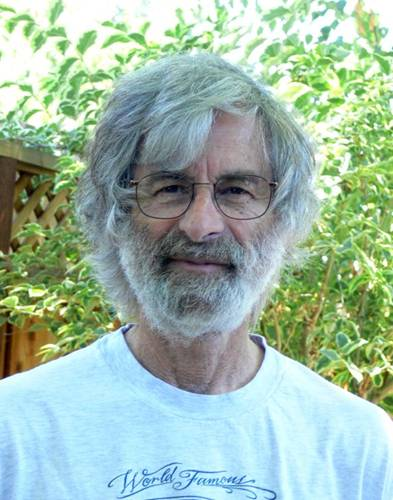
\includegraphics[scale=0.5]{Leslie_Lamport}
 \caption{लेज्लि लॅम्पोर्टचे विकिपीडियावरील छायाचित्र}
 \label{fig:leslie}
 \end{figure}

 \medskip

 \Syn{\7listoffigures}\index{\Syn{\7listoffigures}} ही आज्ञा वापरून पूर्ण दस्तऐवजीतील चित्रांची यादी छापता
 येते. मी ही आज्ञा वापरून चित्रांची यादी या दस्तऐवजाच्या शेवटी छापली आहे.
 \medskip

 \Syn{Tikz} पॅकेज वापरून अतिशय उत्तम प्रतीच्या आकृत्या नि चित्रेही काढता येता.

\section{संदर्भ, निर्देशसूची आणि स्पष्टीकरणकोश}

संदर्भ उद्धृत करणाऱ्या \Syn{\7ref} आणि \Syn{\7cite} आज्ञा वापरताना त्या आधीच्या
शब्दासोबत \(\sim\) वापरून जोडणे फायदेशीर असते.

\subsection{अंतर्गत संदर्भ}
\label{sec:ref}

विविध विभाग, तालिका, चित्रे-आकृत्या, समीकरणे, पृष्ठ आणि याद्यांतील घटकांना {\LaTeX} अंतर्गत संदर्भ
देते. अंतर्गत संदर्भ\index{अंतर्गत संदर्भ| हे पहा {\Syn{\7label}, \Syn{\7ref}}} उद्धृत केला असता, त्या विभागाचा, तालिकेचा, चित्र-आकृत्याचा, समीकरणाचा, पृष्ठाचा
वा याद्यांतील घटकाचा क्रमांक दिसतो.

ज्या बाबीचा संदर्भ द्यायचा आहे, तिच्या \Syn{counter}जवळ
\Syn{\7label\{{\Yvenu संकेत\_शब्द}\}} \index{\Syn{\7label}} असा आठवणीचा शब्द ठेवला
जातो. \textcolor{red}{संकेतशब्द सलग असावा.} ही बाब जर
तालिका, चित्र, आकृती वा यादीतील घटक असेल तर तिला उद्धृत करण्याकरिता
\smallskip

\Syn{\7ref\{{\Yvenu संकेतशब्द}\}} \index{\Syn{\7ref}}
\smallskip

ही आज्ञा; जर पृष्ठ क्रमांक\index{पृष्ठ क्रमांक| हे पहा {\Syn{\7pageref}}} उद्धृत करायचा असेल तर
\smallskip

\Syn{\7pageref\{{\Yvenu संकेतशब्द}\}}; \index{\Syn{\7pageref}}
\smallskip

ही आज्ञा; आणि जर समीकरण क्रमांक\index{समीकरण क्रमांक| हे पहा {\Syn{\7eqref}}} उद्धृत करायचा असेल तर
\smallskip

\Syn{\7eqref\{{\Yvenu संकेतशब्द}\}}\index{\Syn{\7eqref}}
\smallskip

ही आज्ञा वापरली जाते. \Syn{\7eqref} ही आज्ञा एऱ्हवी उपलब्ध नसते. ती हवी असल्यास
कोणत्या पॅकेजची गरज असते?
\medskip

लेज्लि लॅम्पोर्टच्या चित्राच्या \Syn{counter}जवळ मी \Syn{\7label\{fig:leslie\}}
हा आठवणीचा शब्द ठेवला होता. ते चित्र उद्धृत करायचे असल्यास मी
``चित्र\Syn{\(\sim\)\7ref\{fig:leslie\}}'' ही आज्ञा वापरेन. त्याचा परिणाम
``चित्र~\ref{fig:leslie}'' असा दिसतो. हे चित्र असणारे पृष्ठ उद्धृत करण्यासाठी
``\Syn{\7pageref\{fig:leslie\}} ही आज्ञा; तिचा परिणाम
``\pageref{fig:leslie}'' असा आहे. हे उदाहरण पुढीलप्रमाणे वापरता येईल,
\begin{center}
 लेज्लि लॅपोर्टचे छायाचित्र, म्हणजेत चित्रक्रमांक~\ref{fig:leslie} , पृष्ठ ~\pageref{fig:leslie}वर आहे.
\end{center}
\Syn{hyperref} हे पॅकेज वापरून अंतर्गत संदर्भ इलेक्ट्रॉनिक्स स्वरूपात फार
प्रभावीपणे वापरता येतात. मात्र हे पॅकेज फार काळजीपूर्वक वापरावे लागते.

\subsection{बाह्य संदर्भ}

{\Bask \LaTeX}मध्ये \Syn{thebibliography} आणि {\Bask Bib{\TeX}} वापरून
बाह्य संदर्भ\index{बाह्य संदर्भ| हे पहा {{\Syn{thebibliography}, {\Bask Bib{\TeX}}}}}
देण्याच्या पद्धती प्रसिद्ध आहेत; आपण या दोन्ही पद्धती पाहणार आहोत. या दोन्ही पद्धतींत आपले
संदर्भ विशिष्ट प्रकारे एका ठिकाणी साठवावे लागतात. प्रत्येक संदर्भास एक आणि एकच
सांकेतिक शब्दसमूह ठरवला जातो, आणि मग \Syn{\7cite\{{\Yvenu सांकेतिक\_शब्दसमूह}\}}\index{\Syn{\7cite}}
ही आज्ञा मूळ लेखात लिहिताच त्या सांकेतिक शब्दसमूहाशी संबंधित संदर्भ उद्धृत
होतो. \textcolor{red}{संकेतशब्द {\bfseries सलग} असावा}. {\Bask Bib{\TeX}} त्याला दिलेल्या संदर्भांची स्वत: नावानुक्रमे यादी करतो. ही
यादी कालानुक्रमेही करता येते. \Syn{thebibliography}पेक्षा {\Bask Bib{\TeX}} जास्त
प्रमाणात वापरले जाते. संख्येने संदर्भ अवाढव्य असले तरी {\Bask Bib{\TeX}} प्रभावीपणे काम करते.
\medskip

\Syn{thebibliography}\index{\Syn{thebibliography}}करिता दस्तऐवजाच्या शेवटी आणि \Syn{\7end\{document\}}च्या आधी \Syn{thebibliography} वातावरण वापरून संदर्भसूची लिहिली
जाते. संदर्भसूचीतील प्रत्येक संदर्भ \Syn{\7bibitem}\index{\Syn{\7bibitem}} या आज्ञेने सुरू होतो. त्यापुढे \{\} कंस
येऊन त्या कंसात संदर्भाशी संबंधित सांकेतिक शब्दसमूह लिहिला जातो. यापुढे आपणास हवे
त्या प्रकारे आपण संदर्भाचा तपशील लिहू शकता. पुढील \Syn{bibitem} आज्ञा 
किंवा \Syn{\7end\{thebibliography\}} येईपर्यंत हा संदर्भ सुरू राहतो. खाली या
दस्तऐवजात \Syn{thebibliography}च्या उदाहरणादाखल वापरलेल्या संदर्भांचा स्रोत दिला आहे.
\medskip

\Syn{\7begin\{thebibliography\}\{99\}}

\Syn{\7bibitem}\{खंडोबा-ढेरे\} रा.चिं. ढेरे, \Syn{\7textit}\{दक्षिणेचा लोकदेव श्रीखंडोबा\}, पद्मगंधा
 प्रकाशन पुणे, दुसरी आवृत्ती, २४ ऑक्टोबर २०१२, \Syn{ISBN 978-93-82161-25-7}.

 \Syn{\7bibitem}\{गौरी-ढेरे\} रा.चिं. ढेरे, \Syn{\7textit}\{लज्जागौरी\}, पद्मगंधा
 प्रकाशन पुणे, दुसरी आवृत्ती, २१ जुलै २०१५, \Syn{ISBN 978-81-86177-82-2}.

 \Syn{\7bibitem}\{स-बाल\} त्र्यं. बा. ठोमरे, \Syn{\7textit}\{समग्र बालकवी\}, व्हीनस प्रकाशन
 पुणे, पहिली आवृत्ती, सप्टेंबर १९६६. 

 \Syn{\7end\{thebibliography\}}
\medskip

पहिल्या संदर्भात \Syn{bibitem} नंतर कंसात आलेला \emph{खंडोबा-ढेरे} हा शब्द मी या
संदर्भाकरिता सांकेतिक शब्दसमूह म्हणून ठरवला आहे. त्यापुढे मला हवे त्या शैलीत संदर्भाचा
तपशील आला आहे. हा संदर्भ मला इथे उद्धृत करायचा असल्यास मी
\Syn{\7cite\{{\Yvenu खंडोबा-ढेरे}\}} ही आज्ञा वापरेन, आणि हा संदर्भ पुढीलप्रमाणे
दिसेल:~\cite{खंडोबा-ढेरे}. तर \Syn{\7cite}\{गौरी-ढेरे\} आणि \Syn{\7cite}\{स-बाल\}
वापरल्यास \cite{गौरी-ढेरे} आणि \cite{स-बाल} हे दिसेल.
\medskip

सर्व संदर्भांचे तपशिल लिखाणाच्या अखेरीस दिसतात.

\subsubsection{बिबटेक्}

{\Bask Bib{\TeX}}\index{ \Syn{\Bask BibTeX}} वापरताना संदर्भांची यादी एका वेगळ्या दस्तऐवजात करतात. या
दस्तऐवजाच्या नावाच्या अखेरीस \Syn{.bib} असे लिहावे. संदर्भ हा पुस्तक आहे, लेख आहे, प्रबंध
आहे, ग्रंथमालिका आहे, की स्मृतिग्रंथ आहे त्यानुसार त्याचा तपशील भरावा लागतो. प्रत्येक
संदर्भ \Syn{@}ने सुरू होतो. \Syn{thebibliography}च्या वरील उदाहरणातील \emph{खंडोबा-ढेरे} हा संदर्भ हे
पुस्तक आहे; त्याची नोंद \Syn{Dev.bib} असा नवा दस्तऐवज बनवून खालील प्रमाणे केली आहे:
\medskip

\Syn{@book} \{खंडोबा-ढेरे,

\Syn{AUTHOR} = \{रा.चिं. ढेरे\},

\Syn{TITLE} = \{दक्षिणेचा लोकदेव श्रीखंडोबा\},

\Syn{SERIES} = \{\},

\Syn{VOLUME} = \{\},

\Syn{NOTE} = \{\},

\Syn{PUBLISHER} = \{पद्मगंधा प्रकाशन पुणे\},

\Syn{YEAR} = \{२४ ऑक्टोबर २०१२\},

\Syn{PAGES} = \{२१२\},

\Syn{ISBN} = \{\Syn{978-93-82161-25-7}\},

\}\label{page:r-c-dhere-cite}
\medskip

\Syn{@book} नंतर येणारा \emph{खंडोबा-ढेरे} हा या संदर्भाचा संकेतशब्द आहे. जी
माहिती नाहीये, ते रकाने मोकळे सोडले आहेत; संदर्भाबाबत जी माहिती नाहीये, तिचा
उल्लेख अजिबातच केला नाही तरी चालतो. प्रत्येक माहितीच्या शेवटी म्हणजे माहिती संपल्यानंतर स्वल्पविराम
दिला आहे. अधिक लेखक असतील, तर पुन्हा एक \Syn{AUTHOR} = \{नवा लेखक\} ही ओळ
लिहावी. {\Bask Bib{\TeX}}च्या हस्तपुस्तिकेतून प्रबंध, निबंध, अप्रकाशित निबंध,
स्मरणग्रंथ इत्यादींकरिता संदर्भ कसे लिहायचे याची माहिती घ्या.

वरील संदर्भ ज्या दस्तऐवजात उद्धृत करावयाचा आहे, तो दस्तऐवज आणि \Syn{Dev.bib}
एकाच \Syn{folder}मध्ये ठेवावी. लिखाणच्या अखेरीस आणि
\Syn{\7end\{document\}}च्या वर
\medskip

\begin{flushleft}
 \Syn{\7bibliographystyle}\{संदर्भशैली\}

\Syn{\7bibliography\{Dev\}}
\end{flushleft}
\medskip

या आज्ञा लिहाव्यात. पृष्ठक्रमांक ~\pageref{page:r-c-dhere-cite}वरील रा.चि. ढेरे हा संदर्भ उद्धृत करायचा असल्यास, 
\Syn{\7cite\{{\Yvenu खंडोबा-ढेरे}\}} ही आज्ञा वापरावी, आणि दस्तऐवज योग्य
क्रमाने लाटेक्-बिबटेक् इंजिनांवर चालवावा. हा संदर्भ पुढीलप्रमाणे
दिसेल:~\cite{खंडोबा-ढेरे}. \Syn{Dev.bib}मधील केवळ आपल्या लिखाणात उद्धृत केलेले
संदर्भ लिखाणाच्या अखेरीस दिसतात. {\Bask Bib{\TeX}} स्वतः त्यांची आडनावानुसार यादी करते. लक्षात ठेवा की
वरील \Syn{\7bibliography\{Dev\}} या आज्ञेत एरव्ही \Syn{Dev}
ऐवजी आपण ज्या \Syn{.bib} दस्तऐवजात संदर्भ साठवले आहेत त्याचे नाव येते.

\paragraph{संदर्भशैली:}

बिबटेक्-ला कोणत्या शैलीमध्ये संदर्भसूची लिहायची आहे, हे सांगण्याचे काम 
\Syn{\7bibliographystyle} ही आज्ञा करते. \Syn{abbrv, acm, alpha,
 apalike, ieeetr, plain, siam} आणि \Syn{unsrt} या काही संदर्भशैली आहेत. 

\paragraph{लाटेक्-बिबटेक् इंजिनांचा योग्य क्रम:}

 {\Bask Bib\TeX} वापरले असता केवळ एकदा (क्से)लाटेक् इंजिन चालवून यशस्वीरीत्या दृश्य दस्तऐवज निर्माण होत नाही. तर
\begin{center}
 \Syn{(Xe)LaTeX - BibTeX - (Xe)LaTeX - (Xe)LaTeX }
\end{center}
 अशी इंजिने चालवावी लागतात. काहीवेळा इतके करूनही भागत नाही, आणि यशस्वीरीत्या दृश्य दस्तऐवज निर्माण होईस्तोवर खालील क्रमाने इंजिने चालवावी लागतात
 \begin{center}
 \Syn{(Xe)LaTeX - (Xe)LaTeX - BibTeX}
\end{center}

\medskip

\Syn{hyperref} हे पॅकेज वापरून अंतर्गत आणि बाह्य संदर्भ इलेक्टॉनीय स्वरूपात फार
प्रभावीपणे वापरता येतात. मात्र पॅकेज फार काळजीपूर्वक वापरावे लागते.

\subsection{निर्देशसूची}

निर्देशसूची करण्याकरिता \Syn{makeidx} \index{\Syn{makeidx} पॅकेज} पॅकेज वापरावे
लागते. हे पॅकेज वापरल्यावर \Syn{\7makeindex} \index{\Syn{\7makeindex}} ही मूल आज्ञा वापरावी. अणि मूळ दस्तऐवजात जिथे निर्देशसूची हवी आहे
त्या ठिकाणी \Syn{\7printindex} \index{\Syn{\7printindex}} ही आज्ञा वापरून
निर्देशसूची छापता येते.
\medskip

सविस्तर सांगायचे, तर मूलआज्ञासंचामध्ये, म्हणजेच
\Syn{\7documentclass}\{दस्तऐवजाचा प्रकार\} आणि \Syn{\7begin\{document\}}
यांदरम्यान \Syn{\7usepackage\{makeidx\}} ही आज्ञा लिहावी. त्यानंतर मूलआज्ञासंचामध्येच
\Syn{\7makeindex} ही आज्ञा लिहावी. मूळ दस्तऐवजात जिथे निर्देशसूची हवी आहे त्या
ठिकाणी, म्हणजे सहसा \Syn{\7end\{document\}}च्या लगोलग वरती,
\Syn{\7printindex} ही आज्ञा लिहावी.

जो शब्दसमूह निर्देशसूचीमध्ये टाकायचा आहे, त्या शब्दसमूहाजवळ \Syn{\7index}\{निर्देशसूचीमध्ये टाकायचा
 शब्दसमूह\} अशी आज्ञा लिहावी. उदाहरणार्थ
\begin{center}
 ``कर्तरी प्रयोगामध्ये \Syn{\7index}\{कर्तरी प्रयोग\} क्रियापद कर्त्यावर अवलंबून
 असते.''
\end{center}
या वाक्यामध्ये ``कर्तरी प्रयोग'' हा शब्दसमूह निर्देशसूचीमध्ये टाकला
गेला.
\medskip

\Syn{\7printindex} या आज्ञेच्या जागी निर्देशसूची निर्माण होऊन तिथे वर्णानुक्रमे हे
शब्द लिहिले जातात आणि प्रत्येक शब्दासमोर तो ज्या पृष्ठावर आहे त्या पृष्ठाचा क्रमांक
छापला जातो. \Syn{hyperref} पॅकेज वापरले असता, निर्देशसूचीतील शब्दासमोरच्या अंकावर
टिचकी दिली असता, पीडीएफ् वाचकाला थेट त्या पृष्ठावर नेते. \Syn{\7index} या
आज्ञेमध्ये निर्देशसूचीतील एखाद्या मुख्य घटकास कोष्टक क्र. ~\ref{tab:index-com-1}मध्ये
दिल्याप्रमाणे उपघटकही जोडता येतो:
\begin{table}[htb]
 \centering
 \begin{tabular}[htb]{lll}
 \hline
 पृष्ठ क्रमांक & आज्ञा & निर्देशसूचीमधील स्वरूप \\
 \hline
 १२ & \Syn{\7index}\{कर्तरी प्रयोग\} & कर्तरी प्रयोग, १२\\
 १२, २३ & \Syn{\7index}\{कर्तरी प्रयोग\} & कर्तरी प्रयोग, १२, १३\\
 & & \\
 ७ & \Syn{\7index}\{प्रयोग\} & प्रयोग, ७\\
 १२ & \Syn{\7index}\{प्रयोग!कर्तरी\} &\quad कर्तरी, १२\\
 १३ & \Syn{\7index}\{प्रयोग! कर्मणी\} & \quad कर्मणी, १३\\
 \end{tabular}
 \caption{\Syn{\7index} या आज्ञेचे विविध वापर-१}
 \label{tab:index-com-1}
\end{table}

एकाहून अधिक उपघटकही जोडणेसुद्धा शक्य आहे, उदाहरणार्थ, `` शिवकालीन महाराष्ट्रातील पादत्राणे \Syn{\7index}\{शिवकालीन!महाराष्ट्र! पादत्राणे\} ''

एका निर्देशसूचिघटकात दुसरा घटकही उद्धृत करता येतो:

\begin{table}[htb]
 \centering
 \begin{tabular}[htb]{lll}
 \hline
 पृष्ठ क्रमांक & आज्ञा & निर्देशसूचीमधील स्वरूप \\
 \hline
१२ & \Syn{\7index}\{शिवकालीन!महाराष्ट्र! पादत्राणे|&शिवकालीन, १२\\
  &\qquad \qquad हेही
  पहा {महाराष्ट्र, पादत्राणे}\} & \quad महाराष्ट्र\\
  & & \quad पादत्राणे, \emph{हेही पहा} महाराष्ट्र, पादत्राणे\\
 \end{tabular}
 \caption{या आज्ञेचे विविध वापर-२}
 \label{tab:index-com-2}
\end{table}

बिबटेक्-प्रमाणेच निर्देशसूचीकरिताही लाटेक् आणि \Syn{Index} इंजिने योग्य क्रमाने चालवावी
लागतात; हा क्रम पुढीलप्रमाणे:

\begin{center}
 \Syn{(Xe)LaTeX - (Xe)LaTeX - (Make)Index - (Xe)LaTeX }
\end{center}
अशी इंजिने वापरूनही यशस्वीरीत्या दृश्य दस्तऐवज निर्माण न झाल्यास तो निर्माण
होईपर्यंत वरील क्रमाने इंजिने चालवावी लागतात.

\begin{center}
 \fbox{
 \begin{minipage}[htb]{43em}
\Syn{makeidx}ला पर्याय म्हणून बनवलेले \Syn{imakeidx}\index{\Syn{imakeidx}}
पॅकेज कसे वापरायचे हे
शिका. बऱ्याच बाबतीत \Syn{makeidx}पेक्षा \Syn{imakeidx} सरस आहे.
 \end{minipage}}
\end{center}


\subsection{स्पष्टीकरणकोश आणि संक्षेपसूची}

एरव्ही ग्रंथातील संज्ञांचा स्पष्टीकरणकोश\index{स्पष्टीकरणकोश| हेही पहा {चिह्नांचे
 स्पष्टीकरण}} आणि संक्षिप्त स्वरूपात लिहिलेल्या शब्दांची सूची, संक्षेपसूची\index{संक्षेपसूची},
करणे किचकट आणि वेळखाऊ काम असते. मात्र लाटेक्-मधील
\Syn{glossaries}\index{\Syn{glossaries} पॅकेज} पॅकेज हे काम
 लीलया पार पाडते. या पॅकेजचा वापर बिबटेक्-सारखा आहे. याकरिता खालील पायऱ्या
 वापराव्यात:
\begin{enumerate}[leftmargin=*]
\item मूलआज्ञासंचामध्ये, म्हणजेच \Syn{\7documentclass}\{दस्तऐवजाचा प्रकार\} आणि
 \Syn{\7begin\{document\}} यांदरम्यान, \Syn{\7usepackage\{glossaries\}}
 लिहावे; त्यानंतर \Syn{\7makeglossaries}\index{\Syn{\7makeglossaries}} ही आज्ञा लिहावी; ही आज्ञा लाटेक्-ला निर्देशसूची
 बनवण्यास सांगते. \Syn{hyperref} पॅकेज वापरले असल्यास वरील दोन्ही आज्ञा
 \Syn{\7usepackage\{hyperref\}} नंतर लिहाव्यात.
 \medskip
 
 \Syn{\7usepackage\{glossaries\}} या आज्ञेस
 \Syn{xindy}\index{\Syn{xindy}} आणि \Syn{toc} अशी
 दोन प्रचले देता येतात. \Syn{xindy} हे प्रचल वापल्यास, म्हणजेच
 \Syn{\7usepackage[xindy]\{glossaries\}} असे लिहिल्यास,
 \Syn{glossaries} पॅकेज क्सिंडी नामक आज्ञावली वापरून स्पष्टीकरणकोशातील यादी
 बनवतो; क्सिंडी\index{क्सिंडी| हेही पहा {\Syn{xindy}}} वापरण्याचा सल्ला बरेच जण देतात. क्सिंडी न वापरल्यास \Syn{makeidx} वापरून ही यादी बनवली जाते.
\medskip
 
 \Syn{toc} \index{\Syn{toc}} प्रचल वापरले नाही, तर स्पष्टीकरणकोश अनुक्रमणिकेत दिसत नाही. 
 स्पष्टीकरणकोश अनुक्रमणिकेत दाखवायचा असल्यास \Syn{toc} प्रचल वापरावे.
\medskip
 
 वरील दोन्ही प्रचले एकत्र वापरता येतात: \Syn{\7usepackage[xindy, toc]\{glossaries\}} 
 
\item ज्या ठिकाणी स्पष्टीकरणकोश छापायचा आहे, म्हणजेच, सहसा
 \Syn{\7end\{document\}}च्या लगोलग वर, त्या ठिकाणी
 \Syn{\7printglossaries}\index{\Syn{\7printglossaries}} ही आज्ञा लिहावी.
\medskip
 
एरव्ही ``स्पष्टीकरणकोश'' आणि ``संक्षेपसूची'' अशा दोन स्वतंत्र याद्या निर्माण होत
नाहीत तर केवळ स्पष्टीकरणकोश निर्माण होते आणि त्यात संक्षिप्त स्वरूपात लिहिलेल्या
शब्दांचाही अंतर्भाव होतो.
\medskip

संक्षेपसूची वेगळी छापायची असल्यास \Syn{\7usepackage\{glossaries\}}\index{\Syn{\7usepackage\{glossaries\}}} या आज्ञेत
\Syn{acronyms}\index{\Syn{acronyms} प्रचल} हे प्रचल वापरावे, आणि मराठी, हिंदी वा संस्कृतकरिता \Syn{\7renewcommand*\7acronymname}\{संक्षेपसूची\} ही आज्ञा \Syn{\7begin\{document\}}च्या आधी वापरावी\footnote{ ``संक्षेपसूची''ऐवजी आपल्याला हवा असणारा शब्द
 आपण वापरू शकता.}; \Syn{\7renewcommand}च्या वापराकरिता पृष्ठ
 क्र.~\pageref{page:renewcmd} पहा.\label{page:acro-name}
\medskip

स्पष्टीकरणकोश न छापता, केवळ संक्षेपसूची
 छापायची असल्यास \Syn{\7printglossary[type=\7acronymtype]}\index{\Syn{\7printglossary[type=\7acronymtype]}} आज्ञा वापरावी.
 \medskip

स्पष्टीकरणकोशातील केवळ मूळ लिखाणात वापरलेले शब्दच नाही, तर सर्वच शब्द छापायचे
असल्यास \Syn{\7printglossaries} आधी \Syn{\7glsaddall}\index{\7glsaddall} आज्ञा वापरावी.
 
\item आता स्पष्टीकरण हवे असणाऱ्या संज्ञांची यादी कशी करावी आणि त्या कशा
 वापराव्या हे पाहू. स्पष्टीकरण हवे असणाऱ्या संज्ञा संख्येने कमी असतील तर
 \Syn{\7documentclass}\{दस्तऐवजाचा प्रकार\} आणि
\Syn{\7begin\{document\}} यांदरम्यान त्या लिहिता येतात. जर त्या संख्येने खूप
 असतील तर त्या दुसऱ्या एखाद्या \Syn{.tex} दस्तऐवजात लिहाव्यात. हा दस्तऐवज
 आणि मूळ लिखाणाचा दस्तऐवज, ज्यामध्ये या संज्ञा वापरायच्या आहेत, हे दोन्ही एकाच फोल्डरमध्ये
 ठेवावेत. मग मूळ लिखाणाच्या दस्तऐवजामध्ये \Syn{\7documentclass}\{दस्तऐवजाचा प्रकार\} आणि \Syn{\7begin\{document\}} यांदरम्यान \Syn{\7loadglsentries} \{स्पष्टीकरण
 हवे असणाऱ्या संज्ञा लिहिलेल्या \Syn{.tex} दस्तऐवजाचे नाव\}
 \index{\Syn{\7loadglsentries}} \emph{अथवा}
 \Syn{\7input} \{स्पष्टीकरण हवे असणाऱ्या संज्ञा लिहिलेल्या \Syn{.tex}
 दस्तऐवजाचे नाव\} \index{\Syn{\7input}} यांपैकी एक आज्ञा लिहावी. आता या संज्ञा लाटेक् वाचू शकते.
 \medskip
 
 वरीलपैकी एक आणि एकच पद्धत वापरून स्पष्टीकरण हवे असणाऱ्या संज्ञा
 वापराव्यात. या दोन्ही प्रकारांत संज्ञा विशिष्ट पद्धतीने लिहाव्या लागतात; कशा ते
 आता पाहू.
 \medskip
 
 स्पष्टीकरण हवे असणाऱ्या संज्ञा \Syn{\7newglossaryentry}\{संकेतशब्द\}\{तपशील\}\index{ \Syn{\7newglossaryentry}}
 अशा प्रकारे लिहितात. प्रत्येक संज्ञेकरीता, बिबटेक्-मधील संदर्भांप्रमाणे एक आणि एकच
 संकेतशब्द ठरवावा; हा संकेतशब्द\index{संकेतशब्द} वापरून ही संज्ञा उद्धृत करता येते. संज्ञेच्या तपशीलात
 तिचे नाव, स्पष्टीकरण आणि अनेकवचन देता येते. उदाहरणार्थ, फेटा या संज्ञेस खालील
 प्रकारे लिहिता येईल:
 \medskip
 
 \Syn{\7newglossaryentry}\{फे\}
 
\{

\Syn{name}=फेटा,

\Syn{description}=\{पुरुषांसाठीचे शिरस्त्राण म्हणून वापरण्यात येणाऱ्या लांब
कापडास वा त्या शिरस्त्राणास फेटा म्हणतात.\},

\Syn{plural}=फेटे

\}
\medskip

इथे ``फे'' हा संकेतशब्द वा आठवणीचा शब्द आहे. मूळ लिखाणामध्ये \Syn{\7gls}\{फे\}\index{\Syn{\7gls}} ही
आज्ञा वापरून ही संज्ञा स्पष्टीकरणकोशात छापली जाते. उदाहरणार्थ: ``उन्हाळ्याच्या
काळात गावाकडे मुंडासे, फेटे \Syn{\7gls}\{फे\} आणि टोप्या यांचा वापर वाढतो.''

चिह्नांचे\index{चिह्नांचे स्पष्टीकरण} वा त्यांच्या नावांचे स्पष्टीकरण खालील प्रकारे देणे शक्य आहे:
\medskip

\Syn{\7newglossaryentry}\{पाय-गणित\}

\{

\Syn{name}=\{पाय\},

\Syn{description}=\{हा गणितातील एक प्रसिद्ध स्थिरांक आहे. पाय म्हणजे एकक व्यास
 असणाऱ्या वर्तुळाचा परिघ होय.\},

 \Syn{symbol=\{\7ensuremath\{(\7pi) \} \} }

 \}

 वरील उदाहरणाचा वाक्यात वापर फेट्याच्या उदाहरणाप्रमाणेच करतात.
 \medskip

 संक्षिप्त शब्द\index{संक्षिप्त शब्द} आणि त्याचे पूर्ण स्वरूप यांची यादी करताना
 \Syn{\7newacronym} \{संकेतशब्द\} \{शब्दाचा संक्षेप\} \{शब्दाचे पूर्ण स्वरूप\}\index{\Syn{\7newacronym}}
 अशी आज्ञा वापरली जाते. उदाहरणार्थ,
 \begin{center}
 \Syn{\7newacronym}\{दसादशे-व्याज\}\{दसादशे\}\{दरसाल दरशेकडा \}
 \end{center}
 हा शब्द वाक्यात वापरताना खालील आज्ञा वापरल्या जातात
 \begin{table}[htb]
 \centering
 \begin{tabular}[htb]{cl}
 \hline
आज्ञा & दृश्य स्वरूप \\
 \hline
 \Syn{\7gls}\{संकेतशब्द\} & संपूर्ण शब्दसमूह आणि संबंधित संक्षिप्तशब्द\\
 \Syn{\7acrlong}\{संकेतशब्द\} & केवळ संपूर्ण शब्दसमूह\\
 \Syn{\7acrfull} \{संकेतशब्द\} & संपूर्ण शब्दसमूह आणि संबंधित संक्षिप्तशब्द\\
 \Syn{\7acrhort} \{संकेतशब्द\} & केवळ संबंधित संक्षिप्तशब्द\\
 \end{tabular}
 \caption{संक्षिप्तशब्द वाक्यात वापरण्याकरिताच्या विविध आज्ञा}
 \label{tab:acro}
 \end{table}

\item स्पष्टीकरणकोश छापण्याकरिता
 \begin{center}
 \Syn{(Xe)LaTeX - (Xe)LaTeX - Makeglossaries - (Xe)LaTeX}
\end{center}
 अशी इंजिने चालवावी लागतात. काहीवेळा इतके करूनही भागत नाही, आणि यशस्वीरीत्या दृश्य दस्तऐवज निर्माण होईस्तोवर वरील क्रमाने इंजिने चालवावी लागतात.
\end{enumerate}

\section{इतरेतर}

\subsection{सादरीकरणे}

कोष्टक क्र.~\ref{tab:doc-classes}मध्ये नोंदवल्याप्रमाणे लाटेक्-मध्ये बीमर,
\Syn{\Bask Beamer}\index{\Syn{ Beamer}} हा दस्तऐवजाचा प्रकार वापरून सादरीकरणे\index{सादरीकरणे} बनवता येतात. सादरीकरणे बनवणे
हा एक स्वतंत्र आणि विस्तृत विषय आहे. त्याची जुजबी वा तपशीलवार माहिती घेण्याकरिता
वाचकाने, अनुक्रमे, आंतरजालावरील एखादे पुस्तक आणि बीमरची\index{बीमरची} हस्तपुस्तिका
पहावी. बीमरकरिता आतापर्यंत आपण वापरत असलेला मूलआज्ञासंच चालत नसल्याने या
पुस्तिकेत आम्ही केवळ देवनागरीकरिता बीमरचे दोन चौकटी असणारे लहानात लहान उदाहरण\index{बीमरचे उदाहरण} देत आहोत:
\medskip

 \Syn{\7documentclass\{beamer\}}

 \Syn{\7usefonttheme\{serif\}}
 
 \Syn{\7usepackage\{polyglossia\}}
 
 \Syn{\7setdefaultlanguage\{marathi\}}
 
 \Syn{\7setmainfont[Script=Devanagari,Mapping=devanagarinumerals]\{Font
 of your choice; preferably a san-serif one\}}
 \vspace{0.1in}
 
\Syn{\7begin\{document\}}
\vspace{0.1in}
 
\Syn{\7section}\{प्रायोगिक चौकट\}

\Syn{\7begin\{frame\}}

\Syn{\7frametitle}\{पहिली चौकट\} ही पहिली चौकट आहे.

\Syn{\7begin}\{itemize\}

\Syn{\7item}<+-> पहिला मुद्दा

\Syn{\7item}<+-> दुसरा मुद्दा

\Syn{\7item}<+-> तिसरा मुद्दा

\Syn{\7end\{itemize\}}

\Syn{\7end\{frame\}}
\vspace{0.1in}

\Syn{\7section}{लाटेक्-दस्तऐवजाचे स्वरूप}

\Syn{\7begin}\{frame\}
 
\Syn{\7frametitle}\{मूल आज्ञा\}

\Syn{\7begin}\{itemize\}

 \Syn{\7item<+-> \{\LaTeX\}} दस्तऐवजाचे मूलआज्ञासंच आणि लिखाणाचा भाग असे दोन विभाग असतात. मूलआज्ञासंचामध्ये केवळ आणि केवळ आज्ञा असतात, त्यांना मूल आज्ञा असे म्हटले
 जाते.

 \Syn{\7item<+->} हा भाग पूर्णत: तांत्रिक असून असतो.
 
 \Syn{\7item<+->} मूल आज्ञांत दस्तऐवज कसा दिसावा, कोणती पॅकेजे वापरावीत, टंक, भाषा
 कोणती व कशी असावी ही सर्व माहिती साठवलेली असते.

\Syn{\7end\{itemize\}}
 
\Syn{\7end\{frame\}}

\Syn{\7end\{document\}}
\medskip

वाचकांच्या लक्षात आले असेल की, \Syn{\7usefonttheme\{serif\}} ही जास्तीची
मूल आज्ञा बीमरकरिता वापरली आहे.

\subsection{नाट्य-पटकथा-लेखन}

नाट्य-पटकथा-लेखनाकरिता\index{नाट्य-लेखन} \index{पटकथा-लेखन} लाटेक्-मधील ``ड्रॅमॅटिस्ट'', \Syn{dramatist}\index{\Syn{dramatist}}, या पॅकेजचे उदाहरण आम्ही देत आहोत. याकरिता आधी हे पॅकेज प्रस्थापित करावे. ते वापरण्याकरीता, देवनागरी आणि मराठी (वा संस्कृत वा हिंदी, वा इतर भारतीय भाषेच्या) आम्ही दिलेल्या मूल आज्ञा लिहून निबंध, पुस्तक वा स्मरणिका असा तुम्हाला हवा तो दस्तऐवजाचा प्रकार निवडावा. ड्रॅमॅटिस्ट वापरण्याकरिता \Syn{\7usepackage\{dramatist\}} ही मूल आज्ञा लिहावी. हे पॅकेज दृश्यांना, म्हणजेच {\Bask Scene}ना, इंग्रजीत नावे आणि क्रमांक देते. ते बदलण्याकरीता
\smallskip

\noindent \Syn{\7renewcommand\{\7scenename\}\{{\Yvenu दृश्य}\}}

\noindent \Syn{\7renewcommand\{\7thescene\}\{\7arabic\{scene\}\}}
\medskip

या मूल आज्ञा लिहाव्यात (\Syn{\7renewcommand}च्या तपशीलवार माहितीकरिता
पृष्ठ ~\pageref{page:renewcmd} पहा). महत्त्वाचे असे की वरीलपैकी दुसरी आज्ञा
लिहिण्याआधी आपण टंकनिवडीच्या \Syn{\7setmainfont} आज्ञेमध्ये \Syn{Mapping= devanagarinumerals} हे प्रचल वापरले आहे याची खात्री करून घ्या. कारण, वरील नवी आज्ञा ड्रॅमॅटिस्टच्या अंकाना, जे रोमनमध्ये आहेत, अरेबिक करते, आणि टंकनिवडीचे वरील प्रचल मग या अरेबिक अंकांना देवनागरीत आणते.

वरीलपैकी पहिल्या मूल आज्ञेत ``दृश्य''ऐवजी आपण आपल्याला हवा तो शब्दसमूह, उदाहरणार्थ, प्रवेश, टाकू शकता. यानंतर \Syn{\7begin\{document\}} मूळ लिखाण सुरू करावे.

हे लिखाण करताना, \Syn{\7Character}\index{\Syn{\7Character}} आज्ञा वापरून आपल्या पात्रांची ओळख, नावे आणि त्या पात्राकरिता लाटेक्-ला वापरता येईल असा संकेतशब्द देता येतो. मग हा संकेतशब्द वापरून पात्राचे संवाद लिहिता येतात. या आज्ञेचा वापर खालीलप्रमाणे
\smallskip

 \noindent \Syn{\7Character[{\Yvenu पात्रांची ओळख}]\{{\Yvenu पात्रांचे संवाद लेखनात येणारे नाव }\}\{{\Yvenu पात्राकरिता संकेतशब्द}\}}
\medskip

यानंतर \Syn{\7scene}[ ]\index{\Syn{\7scene}} ही आज्ञा वापरून दृश्याची माहिती देता
येते; या आज्ञेनंतर एक मोकळी ओळ सोडावी अन्यथा चूक निर्मांण होऊ शकते असे ड्रॅमॅटिस्टची
हस्तपुस्तिका सांगते. \Syn{\7StageDir}\{ \}\index{\Syn{\7StageDir}} आज्ञा वापरून
नेपथ्याबाबतची माहिती भरता येते. संवाद लेखनाकरिता \Syn{drama}
वातावरण\index{\Syn{drama} वातावरण} वापरले जाते. खालील उदाहरणात पहा,
 \medskip

\noindent\Syn{\7documentclass\{article\}}

\Syn{
\noindent\7usepackage\{fontspec\}

\noindent\7usepackage\{microtype\}

\noindent\7usepackage\{xltxtra\}

\noindent\7usepackage\{polyglossia\}

\noindent\7setdefaultlanguage\{marathi\}

\noindent\7setmainfont[Script=Devanagari,Mapping=devanagarinumerals,StylisticSet=1]\\ \{Yashovenu\}
}

\Syn{
\noindent \7usepackage\{dramatist\}

\noindent \7renewcommand\{\7scenename\}\{{\Yvenu दृश्य}\}

\noindent \7renewcommand\{\7thescene\}\{\7arabic\{scene\}\}
}

\noindent \Syn{\7begin\{document\}}

\noindent \Syn{\7Character[{\Yvenu गोकुळ, विसरभोळे विनोदी पात्र}]\{\7bfseries {\Yvenu गोकुळ}:\}\{Go\}}

\noindent \Syn{\7Character[{\Yvenu शिरस्तेदार, कोर्टातील शिरस्तेदार}]\{{\Yvenu शिरस्तेदार}:\}\{Shir\}}

\noindent \Syn{\7Character[{\Yvenu वकील, जयंतच्या प्रतिपक्षाचा वकील}]\{{\Yvenu वकील}:\}\{Vak\}}

\noindent \Syn{\7scene}[ प्रेमसंन्यास; अंक चवथा, प्रवेश सहावा]

\noindent \Syn{\7StageDir\{

\noindent \7begin\{center\}

\noindent {\Yvenu कचेरीचा देखावा, सर्व मंडळी, साक्षीच्या पिंजऱ्यात गोकुळ.}

\noindent \7end\{center\}

\noindent \}
 }

\noindent \Syn{\7begin\{drama\}}

\noindent \Syn{\7Shirspeaks} ईश्वरसाक्ष खरे बोलेन, खोटे बोलणार नाही.

\noindent \Syn{\7Gospeaks} ईश्वरसाक्ष खरे बोलेन, खोटे बोलणार नाही.

\noindent \Syn{\7Shirspeaks} तुमचे नाव काय ?

\noindent \Syn{\7Gospeaks} गोकुळ.

\noindent\Syn{\7Shirspeaks} बापाचे नाव काय ?

\noindent\Syn{\7Gospeaks} वृंदावन.

\noindent\Syn{\7Shirspeaks} आडनाव ?

\noindent\Syn{\7Gospeaks} विसरभोळे.

\noindent\Syn{\7Vakspeaks} बरे, आता सांगा पाहू, तुमचे वय काय ?

\noindent\Syn{\7Gospeaks} \Syn{\7direct}\{स्वगत\} हं; तोच प्रश्न! आता काय करायचे? नावातल्या अक्षरांना दोन्ही वकिलांनी गुणून त्यात न्यायाधीश मिळवावयाचा? हो, असेच! नाही पण, मला वाटते अक्षरांना न्यायाधीशाने गुणून दोन वकील मिळवावयाचे असे असावे! हं, हेच बरोबर आहे! बारा एके बारा न् दोन चवदा. \Syn{\7direct}\{प्रकट\} चवदा वर्षे!

\noindent \Syn{\7end\{drama\}}

\noindent \Syn{\7end\{document\}}
\bigskip

हे लेखन खालील प्रमाणे दिसेल
\medskip

\Character[गोकुळ, विसरभोळे विनोदी पात्र]{\bfseries गोकुळ:}{Go}
\Character[शिरस्तेदार, कोर्टातील शिरस्तेदार]{शिरस्तेदार:}{Shir}
\Character[वकील, जयंतच्या प्रतिपक्षाचा वकील]{ वकील:}{Vak}

\scene[प्रेमसंन्यास; अंक चवथा, प्रवेश सहावा]

\StageDir{
 \begin{center}
 कचेरीचा देखावा, सर्व मंडळी, साक्षीच्या पिंजऱ्यात गोकुळ.
 \end{center}
}

\begin{drama}
 \Shirspeaks ईश्वरसाक्ष खरे बोलेन, खोटे बोलणार नाही.
 \Gospeaks ईश्वरसाक्ष खरे बोलेन, खोटे बोलणार नाही.
 \Shirspeaks तुमचे नाव काय ?
 \Gospeaks गोकुळ.
\Shirspeaks बापाचे नाव काय ?
\Gospeaks वृंदावन.
\Shirspeaks आडनाव ?
\Gospeaks विसरभोळे.
\Vakspeaks बरे, आता सांगा पाहू, तुमचे वय काय ?
\Gospeaks \direct{स्वगत} हं; तोच प्रश्न! आता काय करायचे? नावातल्या अक्षरांना दोन्ही वकिलांनी गुणून त्यात न्यायाधीश मिळवावयाचा? हो, असेच! नाही पण, मला वाटते अक्षरांना न्यायाधीशाने गुणून दोन वकील मिळवावयाचे असे असावे! हं, हेच बरोबर आहे! बारा एके बारा न् दोन चवदा. \direct{प्रकट} चवदा वर्षे!
\end{drama}
\medskip

वरील उदाहरणात गोकुळकरिता \Syn{Go} असा संकेतशब्द दिला आहे, आणि त्यामुळे गोकुळचे
संवाद लिहिण्याकरिता \Syn{\7Gospeaks} ही आज्ञा वापरली जाते. या उदाहरणात
गोकुळ पात्राच्या नावामध्ये जाड ठसा वापरल्याने काय झाले आहे? \Syn{\7direct}\{ \}
ही आज्ञा काय करते? आपण ड्रॅमॅटिस्टची हस्तपुस्तिका पाहून विविध विभाग निर्माण
करणाऱ्या \Syn{\7act,\7scene,\7Act,\7Scene}, पात्र आणि पात्रसमूह निर्माण
करणाऱ्या \Syn{\7speaker,\7CharacterGroup} या आज्ञा, आणि नेपथ्याशी संबंधित
विविध आज्ञांचा अभ्यास करू शकता.

\subsection{संवादलेखन}

\Syn{dirtytalk} हे पॅकेज\index{\Syn{dirtytalk} पॅकेज} कथालेखकांना संवादलेखनाकरिता उपयोगी पडेल असे
आहे. मूलआज्ञासंचात \Syn{\7usepackage\{dirtytalk\}} लिहिले असता ते कार्यान्वित
होते. ते कार्यान्वित झाले असता, संवाद लिहिण्याकरिता
\Syn{\7say}\{संवाद\}\index{\Syn{\7say}| हे पहा \Syn{dirtytalk} पॅकेज} ही आज्ञा वापरातात.
 उदाहरणार्थ,
 \medskip
 
शिरस्तेदार: \say{तुमचे नाव काय?}

गोकुळ: \say{गोकुळ.}

शिरस्तेदार: \say{बापाचे नाव काय?}

गोकुळ: \say{वृंदावन.}

शिरस्तेदार: \say{आडनाव?}

गोकुळ: \say{विसरभोळे.}
\medskip

 वरीलपैकी पहिल्या वाक्याचे मूळ स्रोतातील लिखाण खालीलप्रमाणे आहे, आणि इतर वाक्ये तशाच प्रकारे लिहिली आहेत:

\noindent
शिरस्तेदार: \Syn{\7say\{{\Yvenu तुमचे नाव काय?}\}}

 \section{काही सल्ले आणि सूचना}
 \begin{itemize}[leftmargin=*]
 \item \Syn{hyperref}\index{\Syn{hyperref}} पॅकेज वापरायला शिका. ते थोडे किचकट असले तरी फार
 उपयुक्त आहे. याच्या वापरामुळे, दृश्य दस्तऐवजामध्ये \Syn{hyperlink} तयार होतात
 आणि एखाद्या \Syn{hyperlink }टिचकी मारताच
 संबंधित पान उघडते. \Syn{hyperref}मुळे इ-पत्ते आणि आंतरजालावरील दुवे सुद्धा
 \Syn{hyperlink}वापरून लिहिता येतात. मात्र, हे पॅकेज वापरताना घ्यावयाच्या
 दोन खबरदाऱ्या अशा, की काही पॅकेजे \Syn{hyperref}च्या आधी लिहावी लागतात
 आणि काही नंतर. हे एकमेव पॅकेज आहे की जे कुठे लिहिले जाते, ते महत्त्वाचे आहे. दुसरी
 बाब अशी की, हे पॅकेज वापरल्यावर विभाग निर्माण करणाऱ्या आज्ञांमध्ये गणिताची
 वातावरणे वापरते येत नाहीत. ती वापरण्याकरिता विशिष्ट पद्घतीने वापरावी
 लागतात, अन्यथा चूक निर्माण होते. \Syn{hyperref}ची हस्तपुस्तिका पाहून ते वापरायला शिका.
 \item सहसा {\Bask PDF}, संकेतस्थळे अशा लाटेक्-स्रोत नसणाऱ्या ठिकाणचा मजकूर लाटेक्-स्रोतात
 चिकटवू नये. लाटेक्-ला {\Bask UTF 8 encoding} असणारा मजकूर मान्य
 असतो. लाटेक्-स्रोत नसणाऱ्या ठिकाणचा मजकूर जर या प्रकारचे {\Bask
 encoding} असणारा नसेल, तर अनाकलनीय चुका निर्माण होतात.
 \end{itemize}
 \subsection{थोडी अधिक माहिती}
\label{sec:info}

\begin{enumerate}[leftmargin=*]
\item {\Bask \TeX}चा उच्चार टेक् असा करतात; {\Bask \LaTeX}चा
 उच्चार लाटेक् अथवा लाटेक् असा करतात. लिहितानाही {\Bask \TeX} आणि {\Bask
 \LaTeX}चे \textit{ स्पेलिंग} {\Bask Tex} आणि {\Bask Latex} असे न लिहिता
 {\Bask TeX} आणि {\Bask LaTeX} असेच लिहितात. \Syn{tex} आणि
 \Syn{latex} ही \textit{स्पेलिंग} तांत्रिक चर्चेमध्ये लिहितात; \cite[{\Bask Section 1.3}]{ll-book} पहा.

\item लेज्लि लॅम्पोर्टने\index{लेज्लि लॅम्पोर्ट} मुळात टेक् ({\Bask \TeX})
 \index{टेक्} या
 आज्ञावलीची (बऱ्याचदा आज्ञावलीस programm वा इंजिन={\Bask
 engine}\index{इंजिन} असेही म्हटले जाते)
 निर्मिती केली; सुंदर दिसणारे गणिती लेख लिहिता यावेत हा त्याचा यामागे उद्देश
 होता. टेक् केवळ अक्षरयोजना ({\Bask typesetting}) करत असे. पुढे, टेक् मधील
 आज्ञा मानवी वापराकरिता जास्त सुलभ असाव्यात म्हणून टेक् वापरूनच लाटेक् ({\Bask
 \LaTeX}) \index{लाटेक् } निर्माण केले गेले. लाटेक्-मध्ये टेक्-च्या आज्ञांचे संच करून, त्यांना मानवी भाषांत शब्दबद्ध केले. उदाहरणार्थ,
 \Syn{\7section} ही लाटेक्-मधील आज्ञा मूलत: टेक्-मधील काही आज्ञांचा संच आहे. पुढे
 जाऊन टेक्-पासून क्सेटेक्, लुआटेक् आणि लाटेक्-पासून लेक्सेटेक्, लुआलाटेक् ही नवी इंजिने बनवली
 गेली.
 
\item लाटेक् शिकण्याकरिता विविध पाश्चिमात्य भाषांत असंख्य पुस्तके आणि लेख उपलब्ध
 आहेत. यापैकी बरेचसे लिखाण आंतरजालावर मोफत उपब्ध आहे. स्वत: लेज्लि लॅम्पोर्टने
 लिहिलेले पुस्तक, \cite{ll-book}, मात्र अतिशय माहितीपूर्ण असून सुलभ आणि खेळकर
 भाषेत लिहिले आहे. हे पुस्तक मोफत नाही. 
\item लाटेक् वापरताना बऱ्याच पॅकेजांची मदत घेऊन काम करता येते. विविध पॅकेजे हा
 लाटेक्-चा अविभाज्य भाग आहे. पॅकेजे लाटेक्-ला प्रचंड शक्तिशाली बनवतात.
\item \label{it:babel-poly} टेक् केवळ अक्षरयोजना ({\Bask typesetting}) करत
 असे. मात्र लाटेक्-पासून त्याला भाषाविचारही देण्यात आले. लाटेक्-मध्ये बेबल ({\Bask
 Babel})\index{बेबल पॅकेज}\index{{\Bask Babel} पॅकेज} हे पॅकेज भाषाविचार निर्माण करते. बेबल आणि लाटेक् मध्ये देवनागरी वापरणे थोडे किचकट
 आहे. शिवाय बेबलमध्ये मराठी भाषाविचार नाहीत. याउलट क्सेलाटेक् आणि लुआलाटेक्-मध्ये
 आपण अभ्यासत असलेले पॉलिग्लॉसिया पॅकेज\index{पॉलिग्लॉसिया पॅकेज} भाषाविचार करते. पॉलिग्लॉसियाला बेबलहून
 अधिक भाषा समजू शकतात आणि ते वापरायला सोपे आहे. ​​पॉलिग्लॉसियामध्ये मराठी व इतर
 भारतीय भाषांकरीता पुरेशा सोयी अजूनही नाहीत. जसा वापर वाढेल, तशा ह्या सोयीही
 निर्माण होत जातील, आणि परिपूर्णही होत जातील.​
\item \label{it:texdoc} लाटेक् प्रस्थापित होताच सर्व प्रस्थापित पॅकेजांच्या
 हस्तपुस्तिकाही\index{हस्तपुस्तिका! पॅकेजच्या}\index{हस्तपुस्तिका} संगणकात येतात.
 एखाद्या पॅकेजची हस्तपुस्तिका पाहण्याकरिता लिनक्स आणि {\Bask OSX Sierra} वर
 टर्मिनल उघडून \Syn{texdoc}<पॅकेजचे नाव>\index{\Syn{texdoc}} ही आज्ञा लिहावी आणि एंटरची कळ
 दाबावी. ताबडतोब ती हस्तपुस्तिका उघडते. उदाहरणार्थ पॉलिग्लॉसियाच्या
 हस्तपुस्तिकेकरिता \Syn{texdoc polyglossia} ही आज्ञा वापरतात. माझ्या माहितीप्रमाण् विंडोज्-वर
 ही आज्ञा बऱ्याचदा चालत नाही. {\Bask CTAN}च्या संकेतस्थळावरही सर्व
 हस्तपुस्तिका उपलब्ध असतात.
 \item कोणता सहाय्यक दस्तऐवज कशासाठी\index{सहाय्यक दस्तऐवज! वापर आणि अर्थ}
 वापरला जातो वा काय माहिती देतो, हे पाहण्याकरिता कोष्टक क्र.~\ref{tab:aux-files} पहा.
 \begin{table}[htb]
 \centering
 \begin{tabular}[htb]{cl}
 \hline
 सहाय्यक दस्तऐवज & काय सांगतो, वा लाटेक् कशासाठी वापरला जातो\\
 \hline
 \Syn{aux} & {\Bask cross-referencing} आणि अनुक्रमणिका,
  चित्र-कोष्टकांची यादी यांकरिता वापरला जातो.\\
 \Syn{log} & लाटेक्-कसे कार्यान्वित झाले याचा पूर्ण तपशील.\\
 \Syn{toc} & अनुक्रमणिकेसंदर्भातील प्रक्रियांचा तपशील.\\
 \Syn{lof} & चित्रांच्या यादीसंदर्भातील प्रक्रियांचा तपशील.\\
 \Syn{lot} & कोष्टकांच्या यादीसंदर्भातील प्रक्रियांचा तपशील.\\
 \Syn{rel} & {\Bask Ref\TeX}ने अंतर्गत आणि बाह्य संदर्भाबाबत केलेल्या
  प्रक्रियांचा तपशील.\\
 \Syn{glo} & पारिभाषिक शब्दावलीची \Syn{\7glossaryentry} ही आज्ञा
  यात असते.\\
  \Syn{blg} & {\Bask Bib\TeX} संदर्भातील प्रक्रियांचा तपशील.\\
 \Syn{bbl} & {Bib\TeX} हा दस्तऐवज निर्माण करते. यात स्रोतामध्ये
  वापरलेले संदर्भ \\ &\Syn{\7bibliography}करिता
    वाचण्यालायक स्वरूपात लिहिले जातात.\\
 \Syn{pdf} & {\Bask PDF} स्वरूपातील दृश्य दस्तऐवज.\\
  \Syn{dvi} & {\Bask DVI} स्वरूपातील दृश्य दस्तऐवज.\\
 \Syn{misfont.log} & टंकांसंदर्भातील चुकांचा तपशील.\\
 \end{tabular}
 \caption{सहाय्यक दस्तऐवज}
 \label{tab:aux-files}
 \end{table}
\end{enumerate}


\newpage

\listoffigures
\listoftables
\printindex

\begin{thebibliography}{99}

\bibitem{स-बाल}
त्र्यं.~बा. ठोमरे.
\newblock {\em समग्र बालकवी}.
\newblock व्हीनस प्रकाशन पुणे, 2000.
\newblock श्रीमती पार्वतीबाई ठोमरे
 संपादित आवृत्ती.

\bibitem{गौरी-ढेरे}
रा.चिं. ढेरे.
\newblock {\em लज्जागौरी}.
\newblock पद्मगंधा प्रकाशन पुणे, २१
 जुलै २०१५.

\bibitem{खंडोबा-ढेरे}
रा.चिं. ढेरे.
\newblock {\em दक्षिणेचा लोकदेव
 श्रीखंडोबा}.
\newblock पद्मगंधा प्रकाशन पुणे, २४
 ऑक्टोबर २०१२.

 \bibitem{ll-book}
{\Bask Leslie Lamport.}
\newblock {\Bask \em {\LaTeX} A Documentation Preparing System, User's
 Guide and Reference Manual}.
\newblock {\Bask Addison-Wesley Publishing Company, 1994}
\end{thebibliography}
\newpage

\begin{flushleft}
 \begin{english}
 {\Bask
 Rohit Dilip Holkar,

 Indian Institute of Science Education and Research Pune,

 Dr.\,Homi Bhabha Road,

 Pashan, Pune 411 008,

 INDIA.

 email: rohit [dot] d [dot] holkar [at] gmail [dot] com.
 \medskip
 
 { \small \emph{\Yvenu लाटेक् आणि पॉलिग्लॉसियाची ओळख} in Marathi and \emph{A
 practical guide to {\LaTeX} and polyglossia for Indian
 Languages} in English, Copyright {\Bask \textcopyright \@} 2017 Rohit Dilip Holkar

 This work may be distributed and/or modified under the
conditions of the LaTeX Project Public License, either version 1.3
of this license or any later version.
The latest version of this license is in
 \url{http://www.latex-project.org/lppl.txt}
and version 1.3 or later is part of all distributions of LaTeX
version 2005/12/01 or later.

This work has the LPPL maintenance status `maintained'.

The Current Maintainer of this work is Rohit Dilip Holkar.

This work consists of the files LaTeX-Mr.tex and LaTeX-Mr.pdf}}
\end{english}
\bigskip

 { \small
रोहित दिलीप होळकर,

भारतीय विज्ञान शिक्षण आणि संशाधन केंद्र पुणे,

डॉ.\,होमी भाभा रस्ता,

पाषाण, पुणे ४११ ००८.

भारत.

इ-पत्ता: {\Bask rohit [dot] d [dot] holkar [at] gmail [dot] com.}

 मराठीमध्ये \emph{\Yvenu लाटेक् आणि पॉलिग्लॉसियाची ओळख} आणि इंग्रजीमध्ये
 \emph{\Bask A
 practical guide to {\LaTeX} and polyglossia for Indian
 Languages}, सर्वाधिकार {\Bask \textcopyright \@} २०१७ रोहित दिलीप होळकर.

 हा दस्तऐवज लाटेक्-प्रकल्प-जन-परवान्याच्या आवृत्ती क्रमांक १.३ वा त्यापुढील कोणत्याही आवृत्तीच्या
 ({\Bask LaTeX Project Public License, either version 1.3 of this
 license or any later version})
 अटींचे पालन करत वितरीत वा/आणि बदलता येणे शक्य आहे. या परवान्याच्या
 आद्ययावत आवृत्तीच्या माहितीकरिता खालील दस्तऐवज पहावा:
 {\Bask \url{http://www.latex-project.org/lppl.txt}}
 आणि आवृत्ती १.३ वा त्यापुढील आवृत्ती (वा आवृत्त्या) या लाटेक्-च्या आवृत्ती २००५/१२/०१ वा पुढील आवृत्त्यांचा
 भाग आहेत.

 या दस्तऐवजाची {\Bask LPPL maintenance} स्थिती {\Bask `maintained'} अशी आहे.

 या दस्तऐवजाचे सध्याचे {\Bask Maintainer} रोहित दिलीप होळकर हे आहेत.

 हा दस्तऐवज {\Bask LaTeX-Mr.tex} आणि {\Bask LaTeX-Mr.pdf} यांनी बनला
 आहे.}
 \end{flushleft}
\end{document}

% Local Variables:
% TeX-engine: xetex
% End:
